\chapter[Introduction to Gravitational waves]{An Introduction to Gravitational Waves, Search Methods and Parameter Estimation Techniques}\label{ch:chap_1}

\hunter{Hey Chris. This chapter is ready for you to review again. I will 
note that I did try to move the GW detection section to the beginning 
of the chapter, but I think there are just too many concepts in there 
that need to be explained first for that to work, so I've left it at the 
end of the chapter.}

\section{General Relativity and Gravitational Waves}

Gravitational waves were predicted by Einstein in his theory of \ac{GR}
well over 100 years ago \cite{GR_Einstein_paper}. In his theory, Einstein 
shows that the more massive an object is, the more curvature in spacetime that object creates. This curvature then has an effect on the motion of objects which encounter it. This effect is summarized succinctly by John 
Archibald Wheeler where he states that ``Spacetime tells matter how to move; matter tells spacetime how to curve''. Curvature may be quantified by first defining a term known as the Riemann curvature 
tensor $R^{\rho}_{\sigma\mu\nu}$. The Riemann tensor describes the change 
experienced by a vector which has been parallel transported over a curved 
manifold\cite{carroll_2019}. Einstein formalises the relationship between matter/energy and the curvature of space-time in his field equations as
%
\begin{equation}\label{eq:FieldEquations}
    G_{\mu \nu} + \Lambda g_{\mu \nu} = \frac{8 \pi G}{c^{4}} T_{\mu \nu},
\end{equation}{}
%
where $\Lambda$ is the cosmological constant (scalar measurement describing the energy density of space), $g_{\mu \nu}$ is the metric which describes the geometric structure of space-time, $G$ is Newton's gravitational constant, $c$ is the speed of light, $T_{\mu \nu}$ is the stress energy tensor which describes the density, direction, and flow of energy in space-time. $G_{\mu \nu}$ is the Einstein tensor defined as
%
\begin{equation}
    G_{\mu \nu} = R_{\mu \nu} - \frac{1}{2} R g_{\mu \nu}
\end{equation}
%
where $R_{\mu \nu}$ is the Ricci curvature tensor (a contraction of the Riemann 
curvature tensor) and $R$ is the Ricci scalar defined as the trace 
of the Ricci curvature tensor. 

%
% Transition towards discussing GWs as small purturbations on the flat spacetime metric
%
The Einstein field equations described by Eq.~\ref{eq:FieldEquations} can  unfortunately only be solved exactly analytically in a limited number of situations. Some solutions include the Schwarzschild solution for a non-spinning singularity (where a singularity is defined as a point in spacetime where 
there is predicted to be infinite curvature~\cite{carroll_2019}) and the Kerr solution for a spinning singularity. 

In the regime of small perturbations 
to spacetime, considering we would like to explore the behavior of non-linear, time-dependent systems in terms of Einstein's field equations, 
we need to put his equations into a more linear form. This can be done by describing the spacetime metric $g_{\mu\nu}$ in terms of an easily computable known solution in flat spacetime with the addition of some small perturbation,
%
% Introduce g_munu
%
where \ac{GW}s may be defined as small perturbations over the curved background spacetime metric $g_{\mu \nu}$. In Euclidean space, the metric (which is what allows us to compute distances or dot products between two point mass objects), is generally described by the identity matrix in Cartesian coordinates. However, in \ac{GR} we have to add the time dimension and in flat spacetime this can be described by the Minkowski metric tensor $\bar{g}_{\mu \nu}$ (sometimes also denoted $\eta_{\mu \nu}$) given by 
%
\begin{equation}
  \bar{g}_{\mu \nu} =   \begin{pmatrix}
-1 & 0 & 0 & 0\\
0 & 1 & 0 & 0\\
0 & 0 & 1 & 0\\
0 & 0 & 0 & 1
\end{pmatrix},
\end{equation}
%
where each column and row represent a dimension of spacetime 
(from left to right and top to bottom: $ct,x,y,z$) where $t$ denotes time, $c$ is the speed of light, 
and $x,y,z$ denote the 
3 spacial dimensions. Time $t$ is negative because the speed 
of light $c$ must remain constant when changing between frames of 
reference \cite{carroll_2019} \hunter{Need Chris to check this}. 
Although the Minkowski metric can be written in non-diagonal 
forms depending on choice of coordinates, this diagonal form 
is chosen because it is computationally easy to invert 
and simple to compute the determinant of the matrix.

Since a \ac{GW} is a perturbation, we can write the metric tensor 
of a small perturbation in flat spacetime as 
%
\begin{equation}
    g_{\mu \nu} = \bar{g}_{\mu \nu} + h_{\mu \nu},
\end{equation}{}
%
where $h_{\mu \nu}(x)$ is the \ac{GW} perturbation tensor ($|h_{\mu \nu}(x) \ll 1|$). 
%Taking the derivative of the metric tensor we arrive at 
%the wave equations, 
%
%\begin{equation}\label{eq:wave_eq}
%    \Box\bar{h}_{\mu\nu} \equiv \Box\bar{h}_{\mu\nu,\alpha}^{\alpha} = 0 
%\end{equation}
%
%where $\Box$ is the  d'Alembertian operator and $\bar{h}_{\mu\nu}$ is 
%a rescaling of the \ac{GW} perturbation tensor in order 
%to simplify Eq.\ref{eq:wave_eq} and may be defined as 
%
%\begin{equation}
% \bar{h}_{\mu\nu} = h_{\mu\nu} - \frac{1}{2}\eta_{\mu\nu}h   
%\end{equation}
%
%One of the well-known solutions to Eq. \ref{eq:wave_eq} is  
%given as 
%
%\begin{equation}\label{eq:gw_plane_solution}
%    h_{\mu\nu} = \textrm{Re}[A_{\mu\nu} e^{ik_{\alpha}x^{\alpha}}],
%\end{equation}{}
%
%where $A_{\mu\nu}$ is the amplitude tensor, $k_{\alpha}$ is the covariant %wavevector and $x^{\alpha}$ is 
%position in spacetime.
%This is also known as the plane wave solution. 
\ac{GW} perturbations are themselves generated by 
accelerating masses which produce 
higher order quadrupole (or multipole) moments~\cite{Maggiore:2007ulw}.

Using $g_{\mu\nu}$, we find that one of the solutions to the linearised 
form of Einstein's field equations may be written as a plane-wave 
solution given by
%
\begin{equation}\label{eq:gw_plane_solution}
    h_{\mu\nu} = \textrm{Re}[A_{\mu\nu} e^{ik_{\alpha}x^{\alpha}}],
\end{equation}{}
%
where $A_{\mu\nu}$ is a complicated amplitude tensor made up 
of multiple independent components and $h_{\mu \nu}$ is a sinusoidal 
wave traveling along the null wavevector $k$~\cite{Maggiore:2007ulw}.

Exploiting guage freedoms~\cite{carroll_2019}, we 
can shift to the Transverse Traceless 
gauge (since this simplifies the plane-wave solution of Einstein's field 
equations to a simplified metric which is only made up of two 
unique components) 
%(since it is convenient to do 
%so given that the metric perturbation is perpendicular to the 
%wavevector in this guage~\cite{Sathyaprakash2009}) 
and $h_{\mu \nu}$ can be rewritten as
%
\begin{equation}
  h_{\mu \nu} =   \begin{pmatrix}
0 & 0 & 0 & 0\\
0 & h_{+} & h_{\times} & 0\\
0 & h_{\times} & -h_{+} & 0\\
0 & 0 & 0 & 0
\end{pmatrix}.
\end{equation}
%
where $h_{+}$ and $h_{\times}$ are representative of the two 
polarization states of a \ac{GW} which are orthogonal to 
one-another~\cite{carroll_2019,Anderson2011}.

%
% h+ and h_cross from a binary system.
%
As derived in~\cite{Capano2011SearchingFG}, assuming that the 
source of the \ac{GW} is emitted from 
a binary astrophysical system with component masses $m_1,m_2$, 
the plus and cross polarization states can 
be expressed as being equivalent to
%
\begin{align}
    h_{+} &\equiv \frac{1}{d} (1 + \mathrm{cos}^{2}\iota) 2\mu(M\Omega^{2/3})
    \mathrm{cos}(2(\Omega t - \phi_0))
    \\
    h_{\times} &\equiv \frac{1}{d} \mathrm{cos}\iota 2\mu(M\Omega^{2/3})
    \mathrm{sin}(2(\Omega t - \phi_0))
\end{align}
%
where $d$ is the distance to the source, $\iota$ is the inclination 
angle of the binary with respect to an observer, $M$ is the total 
mass of the system, $\phi_0$ is the initial phase of the system,  
$t$ is time, $\mu$ is the reduced mass given as $\frac{m_1 m_2}{M}$
and $\Omega$ is Kepler's third law given by
%
\begin{equation}
    \Omega = \sqrt{\frac{M}{a^3}}
\end{equation}
%
where $a$ is the seperation distance between the two component 
masses of the system.

The effect that a passing 
\ac{GW} waveform has on a set of freely floating test particles as 
a function of the waveform's phase $\phi$ for a given polarization state is 
illustrated in Fig. \ref{fig:gw_plus_cross}. This effect on freely floating test masses is what is measured by \ac{LVC} \ac{GW} detectors in the 
form of strain $h$. As shown derived in~\cite{Maggiore:2007ulw}, the 
strain a \ac{GW} induces 
on only two free point masses can be expressed as 
%
\begin{equation}
    h(t) = \frac{2 \Delta L}{L},
\end{equation}
%
where $h(t)$ is the strain amplitude of the \ac{GW} 
as a function of time, $\Delta L$ is 
the absolute change in distance between two point masses induced by the \ac{GW}  and $L$ is the distance between two point masses in the non-presence of a 
\ac{GW}.

For a full derivation concerning the generation and propagation of 
\ac{GW} signals, I refer 
the interested reader to \cite{Flanagan_2005}. Now that we have defined 
how \ac{GW}s propogate and induce strin on freely floating test masses, we 
will introduce in the following section first attempts to detect 
\ac{GW}s, the first indirect observational evidence for \ac{GW}s and 
how the current generation of \ac{GW} detectors function and measure 
\ac{GW} strain $h(t)$.

\begin{figure}
    \centering
    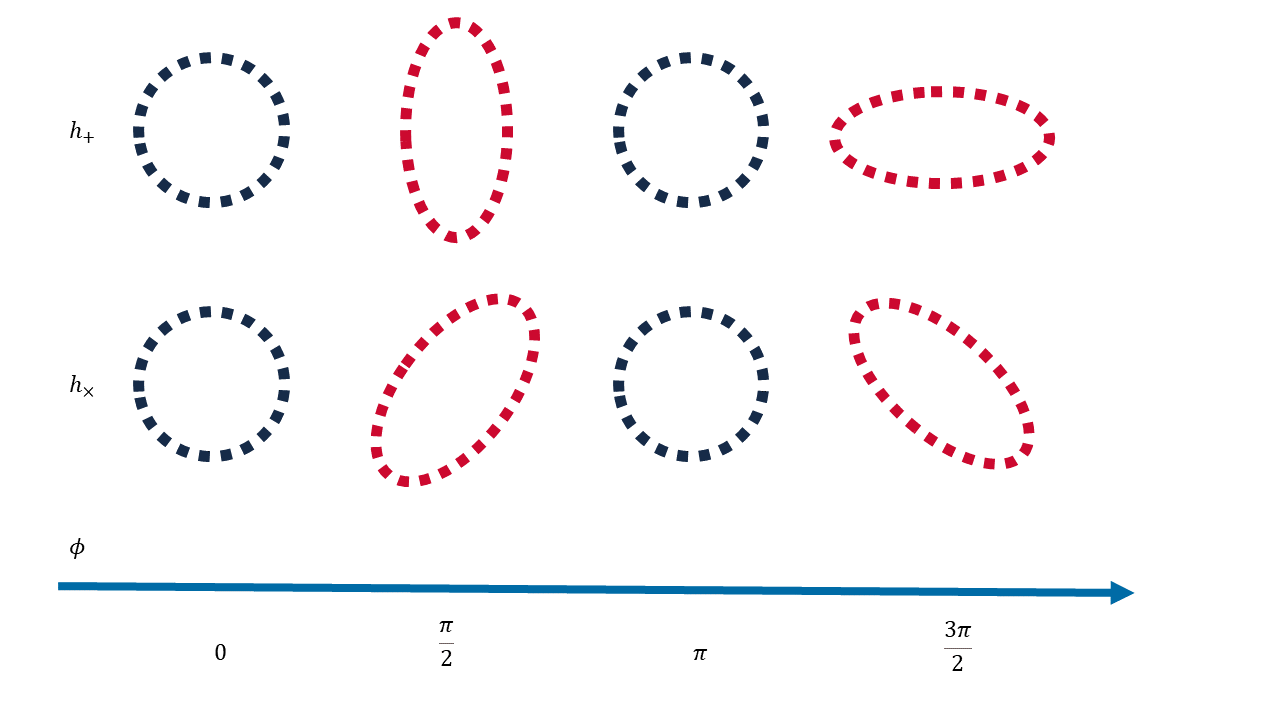
\includegraphics[width=\linewidth]{figures/GW_polarizations_thesis_figure.png}
    \caption[$h_+$ and $h_\times$ polarization illustration]{An illustration of the $h_+$ and $h_\times$ polarizations of a \ac{GW} signal impinging on a set of freely floating test masses as a function of the phase of the \ac{GW} $\phi$ from $0$ to $3\pi / 2$.}
    \label{fig:gw_plus_cross}
\end{figure}

\section{The Weber Bar Detector and the Hulse-Taylor Pulsar}

By the early 1950s technology had progressed enough such that serious 
attempts at experimentally verifying the existence of \ac{GW}s by Einstein were possible. 
One of the earliest and most well-known attempts at doing so was by 
Joseph Weber at the University of Maryland where he used an instrument 
known as a resonant-mass detector (Weber Bar Detector) \cite{PhysRevLett.18.498}
. The Weber Bar 
operates on the principle that when a \ac{GW} impinges on the bar (usually 
made of some type of metal alloy, in this case high Q aluminium~\footnote{Q refers to how underdamped an oscillator is.}) at a 
specific frequency, since the bar is a harmonic oscillator which is driven by the Riemann curvature tensor, it will cause the bar to resonate. If the 
frequency of the \ac{GW} is equivalent 
to the natural resonant frequency of the bar, a \ac{GW} would theoretically be detectable~\cite{PhysRevLett.20.1307}. Weber made the claim in 1968 
that there was 
``good evidence'' for several detections made by his 
experiment~\cite{PhysRevLett.20.1307}, but unfortunately 
no others were able to reproduce his results. Although follow-up results from 
other independent studies were disappointing, 
Weber's work encouraged many others to build their own improved experiments with
breakthrough technological developments at the time and 
kick-started the subsequent field of \ac{GW} detection \cite{1009.1138}. 
Fortunately, in the subsquent years after Weber's 
first published results, there 
would come the first indirect observational evidence for the existence 
of \ac{GW}s.

%
% First indirect observational evidence for GWs
%
In 1975, Russell Hulse and Joseph Taylor made the first direct observation  of a binary pulsar, which subsequently won them the 1993 Nobel Prize in Physics~\cite{1975ApJ...195L..51H}. Booth Hulse and Taylor observed that 
the period of the binary pulsar 
appeared to experience orbital decay as a function of time. The orbital 
decay was thought to likely be attributed to a loss of energy in the 
system due to \ac{GW} radiation predicted by \ac{GR}. The observed period 
decay as a function of time (in years) is represented
in Fig. \ref{fig:hulse_taylor_decay}. As can be seen in the figure, 
there is a striking level of agreement 
between the theoretical decay curve predicted by Einstein's \ac{GR} and 
the observations made by Hulse and Taylor. Importantly, this work was also 
one of the first pieces of indirect observational evidence for the existence of \ac{GW}s. 

\begin{figure}
    \centering
    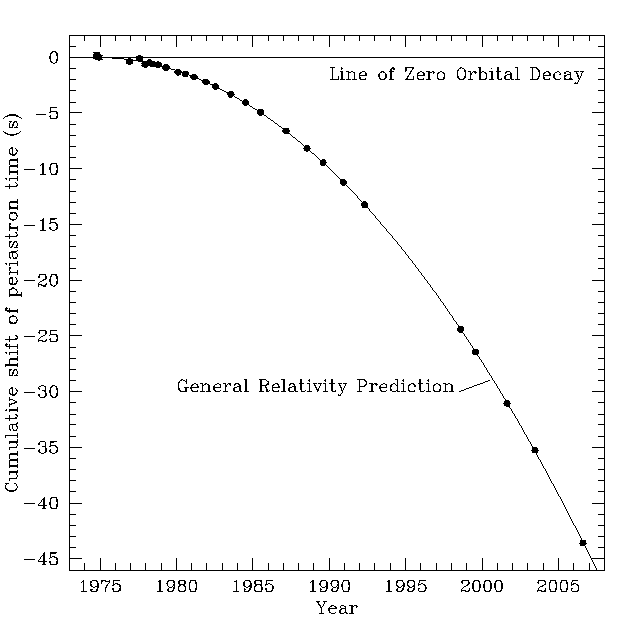
\includegraphics[width=\linewidth]{figures/Hulse_taylor_pulsar.png}
    \caption[Hulse-Taylor binary pulsar decay.]{This figure shows Hulse 
    and Taylor's observations of binary pulsar \texttt{PSR B1913+16} 
    orbital decay as a function of time in years. The orbital decay is quantified by the total cumulative amount the binary system has been offset from it's first observation in 1975 with respect to the binary's perihelion point (black dots). The solid black curve is representative of the theoretical decay curve predicted by \ac{GR}. This figure was produced by the authors of~\cite{1975ApJ...195L..51H}. }
    \label{fig:hulse_taylor_decay}
\end{figure}

Pioneering work by both Hulse-Taylor and Weber, spurred the development 
of advanced \ac{GW} detectors aimed at directly observing 
\ac{GW} events. In the following section we will discuss how the current 
generation of \ac{GW} detectors works and detects \ac{GW}s.

\section{LIGO-Virgo Detectors}

The current generation of \ac{GW} ground-based detectors in 
the \ac{LVC} are composed of 
three observatories, two in North America 
(Hanford, Washington State and Livingston, Louisiana)~\cite{2015} and 
one in Pisa, Italy (Virgo)~\cite{Acernese_2014}. 
There are also other ground-based detectors 
in Hannover, Germany (GEO)~\cite{Affeldt_2014} and Kamioka, Japan 
(KAGRA)~\cite{Akutsu2019}. 
In addition to ground-based detectors there are eventual plans 
to build a space-based observatory called the \ac{LISA}~\cite{1201.3621} which 
will search for super massive \ac{BBH}s (among other 
sources). A 
simplified schematic of the \ac{LVC} detectors is shown in Fig. \ref{fig:detector_schematic}. Each detector (with \ac{LISA} being the 
exception) can be thought 
of as a large-scale Michelson-Morley Interferometer~\cite{Michelson333} 
composed of two arms orthogonal to each other. Each arm of 
the \ac{LIGO} detectors is 4km in length, with the Virgo arms being 
slightly shorter in length at 3km in length.

The detectors operate by first emitting photons from an laser initial 
laser port. 
Photons emitted from the laser pass through a beam 
splitter and down two orthogonal arms of the detectors in 
the form of vacuum sealed beam tubes guided by mirror optics. The photons 
then hit test mass mirrors at both ends
and are caught in what is known as a Fabry-Perot signal recylcing 
cavity~\cite{1899ApJ.....9...87P}. A Fabry-Perot cavity acts to effectively increase the sensitivity of the arms by positively modulating the 
amount of time spent by the light in the arm along, which consequently 
also increases the laser power in the arm~\cite{PhysRevD.75.102002}. After reflecting back and forth in the 
Fabry-Perot cavities, photons are released 
from the Fabry-Perot cavities and return to the beam splitter, subsequently 
recombining and are recorded on a set of photodiodes which measure 
the phase difference between photons from both 
arms. The phase difference information is 
encoded in the interference pattern on 
the readout of the the detector photodiodes, which is the final output of the detectors.

\begin{figure}
    \centering
    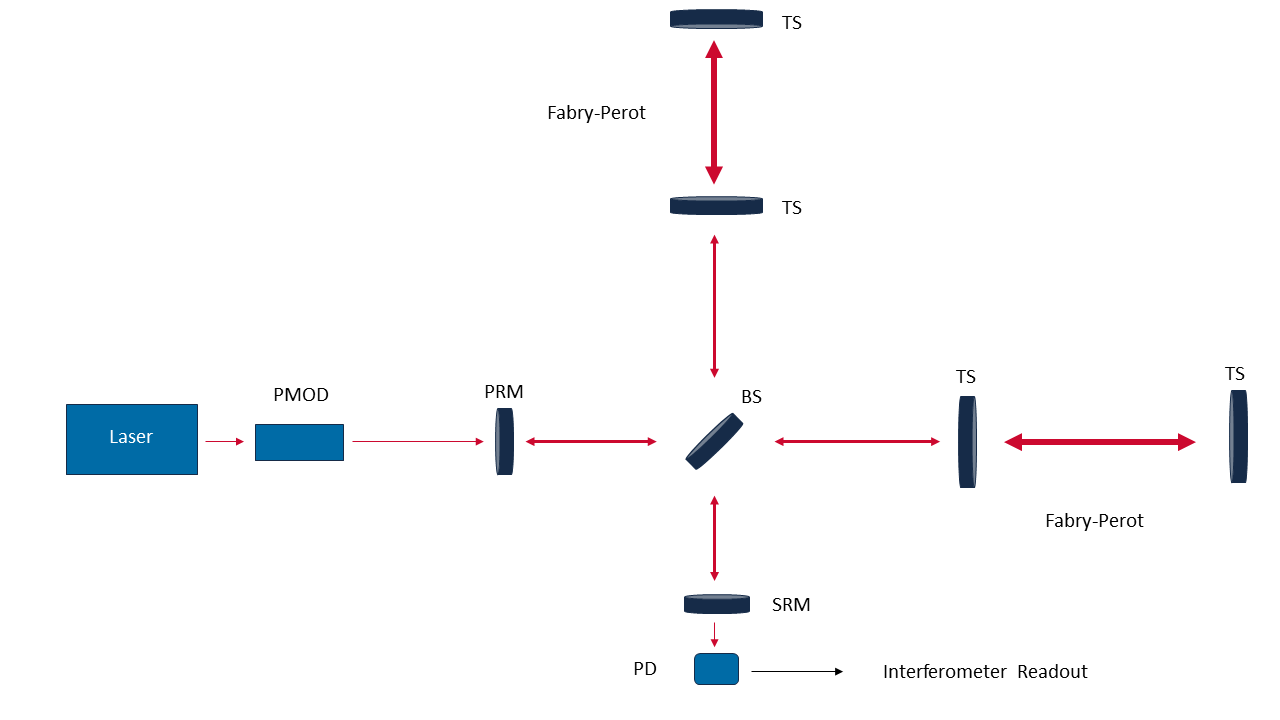
\includegraphics[width=\linewidth]{figures/Interferometer_sketch_figure.png}
    \caption[Illustration of the \ac{LIGO} detectors.]{An illustration of the \ac{LIGO} detectors. A 1064nm laser beam is emitted from a laser on the left-hand side, it then passes through a phase modulator (PMOD) and enters the power recycling cavity (PRM), this effectively boosts the power of the signal. The laser then passes through a beam splitter (BS), which splits the laser beam path into two seperate parts. Each part travels through an input test mass and hits end test masses at the end of both interferometer arms. The beams are then caught in a Fabry-Perot cavity which acts to extend the distance traveled of the beams, as well as the power. In other words, the cavity ``stores'' the photons for a long period ($\sim1$ ms) which allows a potential \ac{GW} signal more time to interact with the photons, thus increasing the sensitivity of the interferometer at low frequencies. Some laser light escapes back down both arms and recombines at the BS where the recombined beam passes through a signal recycling mirror (SRM). Finally, the beam hits a set of photodiodes (PD) which produce the interferometer readout which we use to determine whether or not a \ac{GW} signal is present.}
    \label{fig:detector_schematic}
\end{figure}

Starting from the well-known postulate from relativity that the distance between
two points in spacetime along the path of a light ray traveling 
the $x$ direction may be expressed as
\begin{equation}
    ds^2 = 0 = g_{\mu\nu}dx^{\mu}dx^{\nu}.
\end{equation}
It can be shown through some algebraic manipulation 
(explained in~\cite{SAULSON2013288})
that we can quantify the light travel time difference of photons 
originating from the initial laser port traveling up and down 
the two interferometer arms as 
%
\begin{equation}
    \Delta \tau(t) = h(t) \frac{2L}{c} = h(t) \tau_{rt0}.
\end{equation}
%
where $\tau_{rt0}$ is the return trip time down 
one arm and the phase difference being 
%
\begin{equation}
    \Delta \phi(t) = h(t) \tau_{rt0} \frac{2\pi c}{\lambda}.
\end{equation}
%
Here we can clearly see that the phase difference 
between the two light signals is scaled by the 
length of the interferometer arms $L$. The 
detectors are tuned through control systems such that the photons arriving 
back at the final readout port of the detector act to destructively 
interfere with each other (i.e. create an interference pattern on a dark fringe), where power fluctuations encoded through this interference pattern are recorded on photodiodes. Assuming that a \ac{GW} 
impinges on the detector orthogonal to the plane of the detector and also 
depending on the polarisation state of the wave, 
it will compress one arm 
while stretching the other arm. There will then be a 
detectable difference in phase between the light traveling 
down both arms. Due to this phase difference, the 
light recombining at the beam splitter will no longer 
destructively interfere and a detectable signal will appear 
on the photodetectors in the form of a detectable interference 
pattern~\cite{PhysRevD.95.062003}. In the next section, we will 
discuss how the sensitivity of the detectors may be influenced 
by the orientation of the detectors with respect 
to the \ac{GW} source.

\subsection{Detector Response}

% LIGO antenna patterns
\begin{figure}
    \centering
    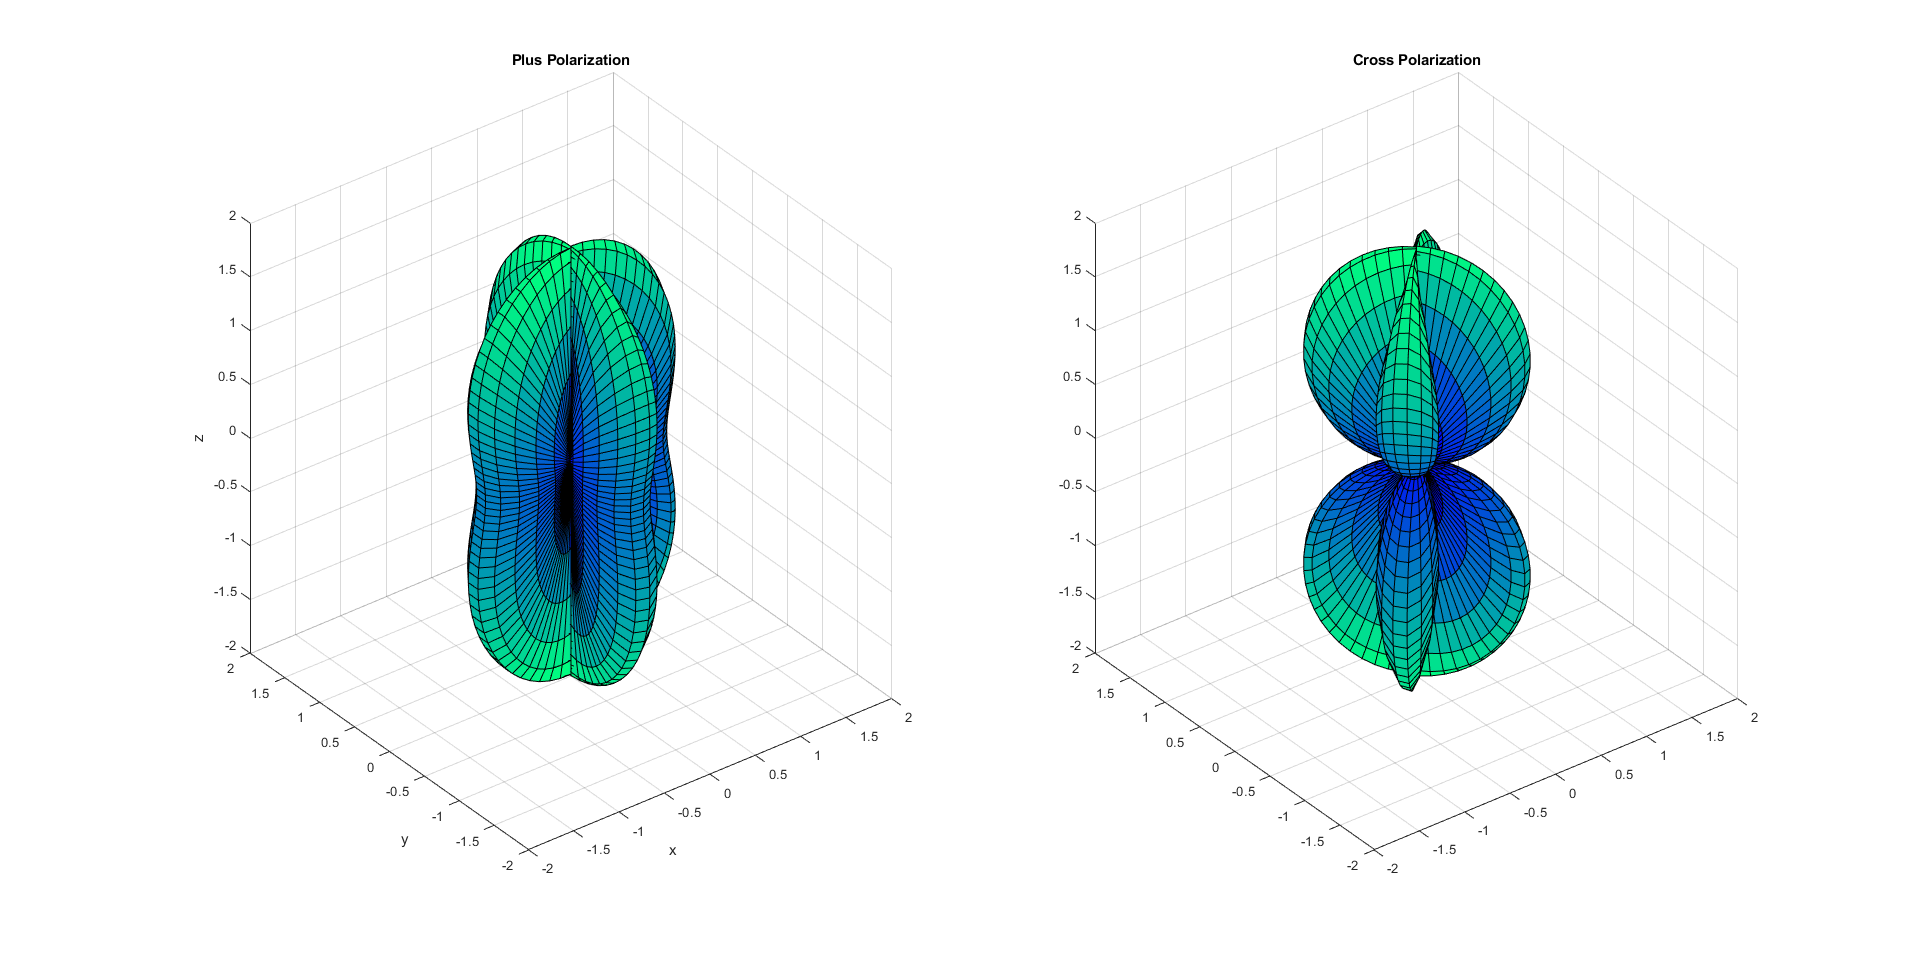
\includegraphics[width=\linewidth]{figures/peanut.png}
    \caption[Illustration of the \ac{LVC} detector antenna patterns for both the $h_\times$ and $h_+$ \ac{GW} polarizations]{An illustration of the \ac{LVC} detector antenna patterns for both the $h_\times$ and $h_+$ \ac{GW} polarizations. The detector itself would lie in the x-y plane with one arm along the x-axis and the other along the y-axis.}
    \label{fig:gw_plus_cross}
\end{figure}

The \ac{LVC} detectors are not equally sensitive to all parts of 
the sky. Mathematically, the sky dependent sensitivity of the detectors 
may be expressed through their antenna patterns. 
The antenna pattern of a detector is dependent upon the location and 
wave polarisation 
of the \ac{GW} source with respect to the detector (with the assumption that the detector is located at the center of a celestial sphere). Changes in the 
antenna pattern have a direct impact on the 
amount of strain measured by the \ac{LVC} detectors. 

As shown in~\cite{PhysRevD.63.042003} and given by 
the derivation shown in~\cite{Capano2011SearchingFG}, the antenna 
pattern may be expressed as
%
\begin{equation}
    \mathrm{F}_{+}^{'} = -\frac{1}{2}(1+\mathrm{cos}^2 \theta) \mathrm{cos}2\varphi \mathrm{cos}2\psi - \mathrm{cos}\theta\mathrm{sin}2\varphi\mathrm{sin}\psi
\end{equation}
%
\begin{equation}
    \mathrm{F}_{\times}^{'} = +\frac{1}{2}(1+\mathrm{cos}^2 \theta) \mathrm{cos}2\varphi \mathrm{sin}2\psi - \mathrm{cos}\theta\mathrm{sin}2\varphi\mathrm{cos}\psi
\end{equation}
%
where $\theta$ is the azimuthal angle, $\varphi$ is the polar angle and $\psi$ 
is the polarisation angle. In other words, $\theta$, $\varphi$ and $\psi$ are all Euler angles which describe the frame of the binary system with 
respect to the detector. The shape of the antenna response is illustrated pictorially in Fig.~\ref{fig:gw_plus_cross} in a Cartesian coordinate system, 
where we can imagine the detector lying along the $x$-$y$ plane. Areas 
where the detector is least sensitive to \ac{GW}s are given by 
the null areas of Fig.~\ref{fig:gw_plus_cross}. 

It is also shown in~\cite{Capano2011SearchingFG} that the 
\ac{GW} strain of both the ``plus'' and ``cross'' polarized portions 
may be generalised for a given polarization angle with respect to the 
direction of \ac{GW} propagation as 
%
\begin{align}
    h_{+}^{'} &= h_{+}\mathrm{cos}2\psi - h_{\times} \mathrm{sin}2\psi \\
    h_{\times}^{'} &= h_{+}\mathrm{sin}2\psi + h_{\times}\mathrm{cos}2\psi
\end{align}
%
Measured \ac{GW} strain is then shown to be expressed as a summation of $h_{\times}^{'}$ 
and $h_{+}^{'}$ attenuated by antenna patterns $\mathrm{F}_{\times}^{'}$ and $\mathrm{F}_{+}^{'}$ given by
%
\begin{equation}
    h(t) = \mathrm{F}_{\times}^{'}(\theta,\psi,\phi)h_{\times}^{'} + \mathrm{F}_{+}^{'}(\theta,\psi,\phi)^{'}h_{+}, \label{eq:measured_strain}
\end{equation}
%
Since the antenna patterns are sky dependent, they are therefore also time dependent. They are time dependent because different detectors will apply different patterns to the same signal, thus altering the received amplitude and phase of the signal. 
For example, very long signals (e.g., \ac{CW} signals) experience time varying antenna responses as the Earth rotates and search methods 
are designed to take this into account~\cite{1712.05897}. In the next 
section, we will discuss how the detectors are also influenced 
by non-astrophysical sources of strain.

\subsection{Detector Noise}\label{sec:detector_noise}

The \ac{LVC} detectors, in addition to being incredibly sensitive to 
strain from \ac{GW} signals, are also sensitive to an abundant number of 
non-astrophysical noise sources. These noise sources can produce 
periods of excess power in measured detector data which may limit 
the sensitivity of the detectors. Some common noise sources include 
gravity-gradient noise, seismic 
noise, thermal noise and quantum shot noise.

%
% Mention PSD 
%
In practice, the performance of the detector may largely be 
characterized by a quantity known as the \ac{PSD}. Assuming the non-presence of 
a \ac{GW} signal, the output of the detector may be assumed to be equivalent to the detector  
noise as a function of time $n(t)$. We define the auto-correlation 
function as 
%
\begin{equation}
    K \equiv E[n(t_1)n^{*}(t_2)],
\end{equation}
%
where $E$ is the expectation value over an ensemble of realisations of 
the noise and $*$ is the complex conjugate. 
Assuming stationary noise, we can write $K$ as being merely dependent 
on $\tau \equiv |t_1 - t_2|$. As shown in ~\cite{Sathyaprakash2009}, 
the \ac{PSD} 
of the detector may thus be written as the fourier transform of the 
auto-correlation function $K(\tau)$ 
%
\begin{equation}\label{eq:PSD}
    S_n(f) \equiv \frac{1}{2} \int_{-\infty}^{\infty} 
    K(\tau) e^{2\pi i f \tau} d\tau, \ f\geq0,
\end{equation}
%
where frequencies are given as being greater than zero. We will now describe 
in detail the types of noise sources which may affect the performance of 
the detector \ac{PSD}.

\begin{figure}
    \centering
    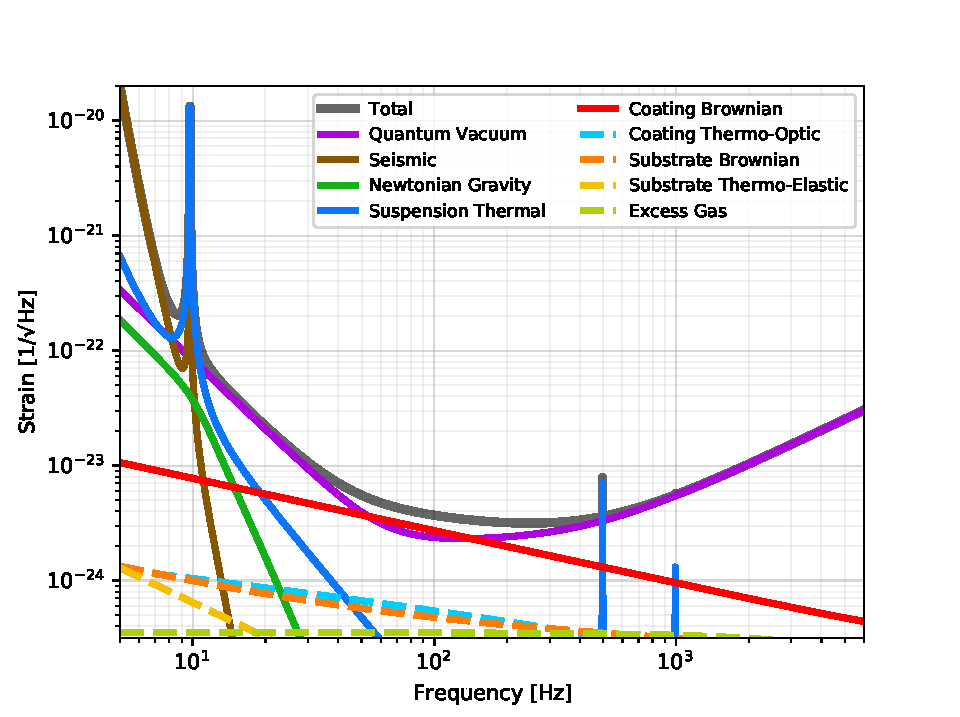
\includegraphics[width=\linewidth]{figures/aLIGO_noise_budget.pdf}
    \caption[Theoretical design sensitivity noise budget curves for Advanced \ac{LIGO}.]{The theoretical design sensitivity noise budget curves for Advanced \ac{LIGO}. As can be seen in the illustration, lower frequencies are largely dominated by seismic motion, mid-range frequencies are 
    dominated by thermal coating Brownian motion on the mirrors as well as quantum vacuum noise between 10 and 100 Hz and higher frequencies are 
    dominated by quantum vacuum shot noise. The plot was generated using the \texttt{pygwinc} computing package \cite{pygwinc}.}
    \label{fig:aligo_noise_budget}
\end{figure}

\subsubsection{Seismic Noise}
%
Seismic noise largely affects the sensitivity of the detectors in the 
low frequency regime ($\sim 10^{-2} -
10^2$Hz~\cite{2012CQGra..29e5006M}) due to a variety of sources 
including: earthquakes, anthropogenic motion and wind. Earthquakes produce 
sets of 
waves (p,s,r-waves) which travel both through the Earth's core/mantel and 
also along the surface of the earth~\cite{Pavlis2003}. 
When one of these seismic waves
hits the detectors they can induce horizontal ground motion on the 
optical components of the detector. In order to isolate the detector 
optics from horizontal ground motion($\sim 0.03 - 0.1$Hz), 
optics are suspended on 
multi-layered seismic isolation stacks~\cite{Matichard_2015}.  
Between $\sim 1 - 3$Hz anthropogenic noise can cause short duration noise 
transients in the detector output. Sources of anthropogenic noise may 
result from individuals walking around in the \ac{LVC} control rooms 
or large trucks passing on a nearby highway~\cite{abbott2016characterization}. 
Wind greater than $10 - 20$Mph can also adversely 
influence the detector sensitvity 
at frequencies of $0.15 - 15$Hz~\cite{Effler_2015}.

%
% Not sure if this is right. 
%
\subsubsection{Thermal Noise}
Thermal noise may be classified into two distinct types: suspension 
and Brownian coating thermal noise and primarily limits detector 
sensitivity in the frequency 
band of $10 - 500$Hz. Suspension noise results 
from thermal motion in the suspension fibers which can induce motion 
into the detector mirrors~\cite{Yamamoto_2002}. 
Brownian coating noise results from 
thermal fluctuations in detector mirror coatings~\cite{Crooks_2006}. 
Both of these sources may be quantified through the application 
of the fluctuation-dissipation theorem as shown in~\cite{Yamamoto_2002}. 
Materials for 
the mirror coatings are chosen such that they have minimal light 
absorption at the wavelength of the laser~\cite{PhysRevD.81.122001}. 
Possible mitigation strategies for reducing thermal noise 
also involve careful choice of coating thickness, as well as the 
use of Cryogenic systems for cooling the suspensions/optics of 
the detector~\cite{2012CQGra..29l4007S}.

\subsubsection{Quantum Noise Sources}
%
% Intro and quantum shot noise
%
There are two sources of quantum noise in the detectors: 
quantum shot noise and quantum thermal radiation pressure 
noise. Both are produced by internal measurement/readout processes.
Quantum shot noise is related to 
from the wave packet-like
behavior of light as it travels through a medium. Since
the distribution of photons arriving within 
a time interval is governed by Poisson statistics,  
we know that the uncertainty on the 
number of photons arriving at the detector 
photodiodes after is proportional to the 
square root of the expected number of photons 
arriving within that same time interval (optical power). 
We can express mathematically the amount of strain induced by shot noise on 
the detectors $h_{\mathrm{S}}$, where subscript $s$ stands for shot noise. 
given by 
%
\begin{equation}
    h_{\mathrm{S}} = \frac{1}{L} \sqrt{\frac{\hslash c \lambda}{2\pi P}},
\end{equation}
%
where $L$ is the arm length of the interferometer, $\hslash$ is 
Planck's constant, $\lambda$ is the laser light wavelength, 
$P$ is the power of the laser and $c$ is the speed of
light~\cite{Hild2014}.

%
% Quantum radiation pressure noise
%
The second type of noise source is quantum radiation pressure noise. Radiation pressure noise arises from the effect of photon momentum transfer onto the test mass mirrors of the detector. When a photon from the detector laser hits a mirror, it transfers some momentum to that mirror. Since all photons do not hit the mirror at the exact same time, there is some variability of pressure exerted on the mirror as a function of time. This moves the mirror in a 
variable manner which leads to a change in the detector arms length and 
thus the noise on the output. This can be mathematically expressed as 
the amount of strain induced on the detector due to radiation pressure 
noise $h_{\mathrm{R}}$ by 
%
\begin{equation}
    h_{\mathrm{R}} = \frac{1}{Lmf^2}  \sqrt{\frac{\hslash P}{2\pi^3 c\lambda}},
\end{equation}
%
where $m$ is the mass of the mirror, $R$ stands for radiation pressure and $f$ is the frequency measured in the \ac{GW} detector~\cite{Hild2014}. 

%
% Possible mitigation strategies
%
Shot noise may be partially mitigated 
through increasing the circulating light power of the laser, since it is 
known that sensitivity of the detector to \ac{GW}s is proportional to the 
laser power, whereas shot noise is proportional to the square root of the 
optical power~\cite{Abadie2011}. Unfortunately, as 
the optical power of the laser is 
increased, so to does thermal radiation pressure noise, which sets 
an effective upper limit on optical laser power in the 
detector. Radiation pressure noise can be reduced by either increasing 
the mass of the mirrors $m$, or the length of the detectors $L$, though 
it should be noted that any increase in either of these values comes 
with added technological and sheer monetary cost constraints.
For a more detailed description of shot noise, see \cite{Hild2014}.

\subsubsection{Gravity-Gradient Noise}

Gravity-gradient noise (or Newtonian noise) is 
noise which results from small stochastic 
perturbations to the gravitational field background in and around 
the \ac{LVC} detector test masses. Some sources of gravity gradient noise 
include: seismic noise and atmospheric fluctuations 
(specifically, changes in air pressure which 
carry with it changes in air density)
\cite{PhysRevD.58.122002}. Gravity-gradient noise decreases steeply with 
increasing frequency and is a primary limiting factor in detector 
sensitivity below frequencies of $1$Hz~\cite{Sathyaprakash2009}.

%%%%%%%%%%%%%%%
%%%%%%%%%%%%%%% 
%%%%%%%%%%%%%%% 
\section{Astrophysical Sources and Search Methods}\label{sec:sources_methods}

There are a variety of sources which produce 
\ac{GW} signals. Most are not large enough to be seen by the 
\ac{LVC} detectors, but some astrophysical sources 
are indeed sufficiently strong enough 
to be detected. Such detectable signals may be categorized into 4 
distinct types including: \ac{CBC}, burst,
continuous and 
stochastic \ac{GW}s. In this 
section I will explain in detail the unique characteristics which 
describe each of these signal types. I will also 
describe several methods used by the 
\ac{LVC} to search for signals from \ac{CBC}, \ac{GW}, burst and 
stochastic \ac{GW}s.

\subsection{Compact Binary Coalescencs}\label{sec:CBC_source}

\ac{CBC} signals arise from the collision of massive 
( of order $\sim M_{\odot}$) compact 
binary objects (such as \ac{BH}s and \ac{NS}s) moving at high relativistic speeds. \ac{NS}s may be defined as being 
the leftover cores of dead stars which have 
exploded in a supernovae and then collapsed down into an object roughly 
the mass of our sun and with a radius of a few 
km. \ac{CBC} systems can 
include \ac{BBH}s, \ac{NSBH} pairs, \ac{BNS}s and super massive \ac{BH} encounter events.
A \ac{CBC} signal waveform is made up of three components: the inspiral, merger 
and ringdown phase and can be approximated using a combination 
of post-Newtonian theory~\cite{PhysRevD.84.049901,PhysRevD.80.084043,Blanchet2014,PhysRevD.93.084054},
the effective-one-body formalism~\cite{PhysRevD.59.084006}, and numerical
relativity simulations~\cite{PhysRevLett.95.121101}.

%
% How each signal type is parameterized
%
\ac{BBH} signals are parameterised by 15 different parameters (discounting 
eccentricity). Two of these  
parameters describe the two component masses of 
each compact object in the binary system ($m_1$,$m_2$) and are sometimes 
commonly combined in an expression known as the chirp mass given by 
%
\begin{equation}
    M_c = \frac{(m_1 m_2)^{3/5}}{(m_1 + m_2)^{1/5}}.
\end{equation} 
%
Other parameters include: the time at which the binary coalesced, luminosity distance, phase of the waveform at coalescence, sky 
location (right ascension, declination), 
inclination angle, polarization angle, spin magnitudes, tilt angles, 
azimuthal angle and azimuthal position. \ac{BNS} and \ac{NSBH} 
events are also parameterized by the 
same \ac{BBH} parameters mentioned above, but their waveform is 
additionally impacted by the internal structure of the \ac{NS}. The 
affect the \ac{NS} internal structure has on the \ac{GW} waveform 
may be parameterized in the form of 
additional tidal parameters given in ~\cite{PhysRevD.81.123016}. 

As the two objects rotate about each other, energy is radiated away in the form of \ac{GW}s primarily due to the mass quadrupole moment of the binary system
~\cite{Maggiore:2007ulw}. 
Over the course of millions or even billions of years, the two objects will inspiral in towards each other~\cite{10.3389/fspas.2020.00038}. As the orbital separation decreases, the objects will move faster and increasingly
radiate away more and more energy in the form \ac{GW}s. This is known 
as the inspiral phase where the frequency of the \ac{GW} waveform 
increases as a ``chirp-like'' signal. Prior to merging, the objects release a tremendous amount of energy, producing 
peak luminosities equivalent to $\mathcal{O}(1 \times 10^{56}\mathrm{erg \ s^{-1}})$
, making \ac{CBC} signals some of the most luminous events in 
the universe~\cite{1811.12907,2010.14527}. 
If the objects are \ac{BBH}s, they 
will merge and coalesce into a single perturbed \ac{BH} which emits \ac{GW}s at 
a set of frequencies which is parameterised by the remnant single black 
hole total mass and spin angular momentum~\cite{Hawking1972,PhysRev.164.1776,
PhysRevLett.26.331}(also known as the 
``ringdown'' phase of the \ac{GW} signal). If the objects are \ac{BNS}s 
they will typically collide and are thought to generate short \ac{GRB}s followed by a kilonovae~\cite{2017arXiv171005834L}. Importantly, both the short 
\ac{GRB} and kilonovae components may be measured by other \ac{EM} telescopes across the spectrum. Theoretically, \ac{NSBH} events should also be able
to produce \ac{EM} radiation, but this is 
largely dependent on several factors including the mass ratio of the 
binary system, \ac{BH} spin and \ac{NS} radius~\cite{doi:10.1146/annurev-nucl-102115-044819}.

% f_ISCO explanation
The frequency near which the two objects will merge (and the point 
at which the frequency of the \ac{GW} waveform stops increasing) is 
largely a function of a quantity known as the  
innermost stable circular orbit $R_{\mathrm{ISCO}}$. This radius is the distance between two compact objects in orbit at which their motion becomes unstable and the two objects rapidly decrease their radial distance between each other. The radius at which this occurs is defined as 
%
\begin{equation}
    R_{\mathrm{ISCO}} = \frac{6GM}{c^2},
\end{equation}
%
where $G$ is the gravitational constant, $M$ is the total mass of 
the system, and $c$ is the speed of light. The corresponding frequency at which the orbit becomes unstable may be estimated using Kepler's third law and can be expressed as 
%
\begin{equation}
    f_{\mathrm{ISCO}} = \frac{1}{T} \lesssim 
    \sqrt{\frac{GM}{4\pi^2R^3_{\mathrm{ISCO}}}} \simeq 2.2 \mathrm{kHz}\frac{M_\odot}{M} ,
\end{equation}
%
where $T$ is the period of the orbit and $M$ is the total mass of the system~\cite{Maggiore:2007ulw}. Now that we've characterised \ac{CBC} 
signals, we will describe data analysis methods used for detecting 
\ac{CBC} signals.


\subsection{Compact Binary Coalescence Search Method}

The measured strain (output) of the \ac{LVC} \ac{GW} detector is given as a 
time series $s(t)$ produced by the resulting phase shift of the detector laser beam. Due to the fact that
the detector is not perfectly isolated from all non-astrophysical sources, the output of the detector when a \ac{GW} is present will be a combination of 
both the astrophysical strain directly  
from the \ac{GW} $h(t)$ as a function of time, as well as the noise $n(t)$ 
which is a combination of all other forms of non-astrophysical strain in the 
detector also as a function of time
%
\begin{equation}\label{eq:alternate_hypo}
    s(t) = h(t) + n(t).
\end{equation}{}
%
If no signal is present, the measured strain of the detector 
is simply equivalent to the noise $s(t) = n(t)$. This is generally known 
as the null hypothesis $H_0$. We define Eq.~\ref{eq:alternate_hypo} as the alternative hypothesis $H_1$. We assume that the noise is governed by 
a stochastic process and the joint-probability 
distribution $p(n)$. The noise is also assumed to be both stationary and 
Gaussian, where stationarity is defined as the noise  
having constant statistical properties as a function of time 
and Gaussianity dictates that noise 
samples are distributed such that their joint-probability distribution 
has mean of 0 and a standard deviation of 1. In the frequency domain, 
stationarity is defined as noise being uncorrelated across frequency bins and 
Gaussianity as each noise frequency bin following a Gaussian 
distribution~\cite{Abbott_2020}. 
In reality this is a poor approximation of the detector noise, where the noise
is 
more likely to be non-Gaussian and non-stationary. For those cases where there 
is non-Gaussianity various glitch identification tools and techniques are 
used to identify periods of excess noise in the detector data
output $s(t)$~\cite{Abbott_2020,2021CQGra..38m5014D,0264-9381-34-6-064003,
2018RSPTA.37670286N,abbott2016characterization}.

Given Gaussian noise, our problem then becomes, how does one distinguish noise from actual \ac{GW} signal? Fortunately, the problem of extracting low \ac{SNR} signals from the background is not uncommon in physics and the field of statistics and may be accomplished through a technique known as matched 
filtering.

\subsubsection{Matched Filtering}\label{sec:matched_filtering}

The primary method for detecting \ac{CBC} signals is through 
matched filtering~\cite{PhysRevD.60.022002}. 
Matched filtering has been applied in a variety of contexts outside of \ac{GW} 
astronomy including: radar/sonar~\cite{WOODWARD1953100} and digital 
communications~\cite{doi:10.1080/00207217408900375}. In this subsection, 
I will describe how matched filtering is used within the context of 
\ac{GW} detection of \ac{CBC} signals including deriving the 
optimal matched filter, explanation of additional statistical 
tests such as the $\chi^2$ statistic, as well as
a discussion on template bank generation and coincidence testing.

%
% Brief aside on waveform modeling
%
To start, we can take advantage of the fact that we generally have a good understanding of the form of $h(t)$ through a combination of analytic and numerical waveform modeling. 
% PN stuff
At large distances between the two compact 
objects of the binary system and velocities which are smaller 
than the speed of light $v \ll c$ (slow motion, weak-field), 
a \ac{PN} approximation may be used to model the \ac{GW} 
waveform, as outlined in~\cite{Will5938,Blanchet2014}. 
% Numerical solutions
However, at smaller separation distances, 
this approximation is not valid and computationally expensive 
numerical solutions to Einstein's field equations are 
then required through \ac{NR}~\cite{Cardoso2015}. Modeling 
the entire waveform requires stitching together both \ac{PN} 
and \ac{NR} estimates in a semi-analytic 
approximate of the entire waveform. 
The two main approaches currently used to model the 
\ac{IMR} phases of the whole signal use either the 
\ac{EOB} formalism~\cite{PhysRevD.89.061502} (SEOBNR waveform family) or the 
\ac{Phenom} framework~\cite{PhysRevD.93.044006,PhysRevD.93.044007} 
(IMRPhenom waveform family). For further 
details and an overview of \ac{GW} waveform modeling 
see ~\cite{10.3389/fspas.2020.00028}.

%
% New and improved matched filtering derivation 
%
Given that we have an accurate understanding 
of \ac{GW} waveforms through 
waveform approximation techniques, we will derive an algorithm 
for testing the alternative hypothesis $H_1$ of whether or not a signal is 
present in the detector noise. We will be following the derivation 
found in ~\cite{Anderson2011}. In order to do this we must 
first define the likelihood ratio given by 
%
% Odds ratio
\begin{equation}\label{eq:likelihood_ratio}
    \Lambda(B|A) \coloneqq \frac{P(A|B)}{P(A|\neg B)},
\end{equation}
%
where $\Lambda(B|A)$ is the likelihood of $B$ given $A$, 
$P(A|B)$ is the conditional probability of $A$ given $B$ 
and $P(A|\neg B)$ is the conditional probability of $A$ 
given $B$ is not true where $P(\neg B) = 1 - P(B)$.
If we want to find the likelihood of the alternative 
hypothesis $H_1$, given the measured strain output of the 
detector $s$, we can substitute this into Eq.~\ref{eq:likelihood_ratio} 
and rewrite as
%
\begin{equation}\label{eq:altern_likelihood}
 \Lambda(H_1|s) = \frac{p(s|H_1)}{p(s|H_0)}    
\end{equation}
%
where $p$ is representative of a probability density. We also define  
the probability density of a Gaussian $p_G(s)$ as a function 
of time series $x$ as 
%
\begin{equation}\label{eq:Gaussian_tseries_dist}
    p_{G}(x) = \frac{1}{\sigma\sqrt{2\pi}} 
    e^{-\frac{1}{2} \left(\frac{(x-\mu)}{\sigma}\right)^2}
    \ \propto \ e^{-\frac{1}{2}\langle x,x \rangle},
\end{equation}
%
where $\mu$ is the mean of the time series distribution, $\sigma$ is 
the standard deviation of the time series distribution and $\langle x,x\rangle$ is 
the inner product of the time series $x$. Given 
Eq.~\ref{eq:Gaussian_tseries_dist} and acknowledging 
that Eq.~\ref{eq:alternate_hypo} may be rewritten as 
$n(t) = s(t) - h(t)$ under $H_1$ and as $n(t) = s(t)$ under 
the null hypothesis $H_0$, we can substitute Eq.~\ref{eq:Gaussian_tseries_dist} 
into Eq.~\ref{eq:altern_likelihood} under the two different hypotheses 
$H_0,H_1$ and write as 
%
\begin{equation}
    \Lambda(H_1|s) = \frac{e^{-\frac{1}{2}\langle s-h,s-h \rangle}}
    {e^{-\frac{1}{2}\langle s,s\rangle}}.
\end{equation}
%
expanding we arrive at 
 \begin{align}
    \Lambda(H_1|s) &= \frac{e^{-\frac{1}{2}\left(\langle s,s\rangle -2\langle s,h\rangle +\langle h,h\rangle \right)}}
    {e^{-\frac{1}{2}\langle s,s\rangle }} \\
    \\
    &= \frac{\frac{e^{\langle s,h\rangle }}
    {e^{\frac{\langle s,s\rangle }{2}}e^{\frac{\langle h,h\rangle }{2}}}} 
    {\frac{1}{e^{\frac{\langle s,s\rangle }{2}}}} 
    = \frac{e^{\langle s,h\rangle } e^{\langle s,s\rangle /2}}
    {e^{\langle s,s\rangle /2}e^{\langle h,h\rangle /2}} \\
    \\
    &= \frac{e^{\langle s,h\rangle }}{e^{\langle h,h\rangle /2}}\label{eq:final_mf_like} 
    = e^{\langle s,h\rangle } e^{-\frac{\langle h,h\rangle}{2}},
 \end{align}
%
where in Eq.~\ref{eq:final_mf_like} we see that observed 
data in the detector $s$ influences the likelihood strictly  
through the inner product $\langle s,h\rangle$. Given the relation
%
\begin{equation}
    \langle a,b\rangle \equiv 2 \int_{0}^{\infty} \frac{df}{S_n(f)} 
    \left( \tilde{a}(f)\tilde{b}^{*}(f) + 
    \tilde{a}^{*}(f)\tilde{b}(f)\right)
\end{equation}
%
stated in ~\cite{Sathyaprakash2009}, where $\tilde{a}$ 
represents the Fourier transform of $a$,
we can say that the the most optimal expression for determining 
whether $H_1$ is true may be expressed through the inner product 
$\langle s,h\rangle$ as
%
\begin{align}
    \langle s,h\rangle &= 2 \int_{0}^{\infty} \frac{df}{S_n(f)} \left(
    \tilde{s}(f)\tilde{h}^{*}(f) + 
    \tilde{s}^{*}(f)\tilde{h}(f)\right). \\
    &= 4 \int_{0}^{\infty} \frac{\tilde{s}(f) \tilde{h}^{*}(f)}
    {S_{n}(f)} df,\label{eq:opt_mf} 
\end{align}
%
where $\tilde{s}(f)$ is the fourier transform of the detector output and  
$\tilde{h}(f)$ is the fourier transform of the \ac{GW} strain. Dividing 
Eq.~\ref{eq:opt_mf} by the magnitude of the waveform $\sqrt{\langle h,h\rangle }$ 
gives the \ac{SNR} $\rho$~\cite{PhysRevD.85.122006}, where the greater the 
value of $\rho$, the more likely a given \ac{GW} 
waveform $h(t)$ is in the detector output $s(t)$.

We also maximise over the phase of the template 
waveform, whereby each template waveform has 
orthogonal phase components $h_{\mathrm{sin}}$ 
and $h_{\mathrm{cos}}$. As shown in~\cite{PhysRevD.85.122006}, after maximising over 
phase we arrive at 
\begin{equation}
    \rho^2 = 
    \frac{\langle s,h_{\mathrm{sin}}\rangle ^2}{\langle h_{\mathrm{sin}},h_{\mathrm{sin}}\rangle } + 
    \frac{\langle s,h_{\mathrm{cos}}\rangle ^2}{\langle h_{\mathrm{cos}},h_{\mathrm{cos}}\rangle } = 
    \frac{\langle s,h_{\mathrm{sin}}\rangle ^2 + \langle s,h_{\mathrm{cos}}\rangle ^2}{\langle h_{\mathrm{sin}},h_{\mathrm{sin}}\rangle }
\end{equation}
where $\rho^2$ is known as the matched filter \ac{SNR}. The matched filter 
\ac{SNR} is the primary statistic used to determine if a template is a good 
match for a given detector output $s(t)$. If $\rho^2$ is above a 
pre-determined threshold using a given template waveform $h(t)$, at a 
specific time $t$, we 
say that this period in the observed data is a \textit{trigger}. There are also 
additional statistical tests performed, such as the the $\chi^2$ test, 
which will be discussed later. 
%
% Discuss templates and template bank placement
%
%Since there are a range of parameters which may describe 
%$h(t)$, we are now left with the decision on how to 
%sample from this parameter space. 
%As shown in ~\cite{PhysRevD.71.062001}, $h$ may 
%be parameterised by  
%
%\begin{equation}
% h(t) = \frac{D}{d} \left(\mathrm{cos}\phi h_{\mathrm{cos}}(t-t_0)
% +\mathrm{sin}\phi h_{\mathrm{sin}}(t-t_0)\right),
%\end{equation}
%
%the effective distance of the source,   
%$h_{\mathrm{sin}}$ and $h_{\mathrm{cos}}$ are the two orthogonal 
%phases of $h(t)$~\cite{FindChirp}, $d$ is the 
%effective distance from the source, $t_0$ is the time of coalescence 
%of the binary at merger and $\phi$ is the phase. Parameters $d,t_0,\phi$ (henceforth collectively denoted as 
%$\gamma$) are unknown in practice. The effective distance from the source 
%$d$ is unimportant with regards to matched filtering since it simply sets 
%a scale for the matched filter output. We can determine the best 
%matching phase $\phi$ for given template waveform $h(t)$ by maximising 
%over the phase $\phi$. After maximising over phase, we arrive at the 
%matched filter 
%we 
%typically marginalize out these \textit{nuisance} parameters by first  
%defining the likelihood ratio
%
%\begin{equation}\label{eq:mf_unknown_par_like}
%    \Lambda(H_{\gamma}|s) = \frac{p(s|H_\gamma)}{p(s|H_0)},
%\end{equation}
%
%where by using the marginalized likelihood it is shown 
%in ~\cite{Anderson2011} that 
%
%\begin{equation}\label{eq:max_like_mf}
%    \left <s - h(\gamma), \frac{\partial}{\partial\gamma_i} h(\gamma)\right> 
%    \bigg\rvert_{\gamma=\gamma_{\mathrm{max}}} = 0. 
%\end{equation}
%
%\hunter{I think this is an inner product, but not sure.}By solving %Eq.~\ref{eq:max_like_mf} for many \ac{GW} templates $i$ 
%with parameters $\gamma$ for $\gamma_{\mathrm{max}}$, one can find 
%a set of templates which maximizes the likelihood of Eq.~\ref{eq:mf_unknown_par_like}. 

%
% Template bank placement
%
Choosing how to sample \ac{GW} templates from the vast 
parameter space which best match $h(t)$ can be 
challenging. This is typically done by first constructing 
what is known as a \textit{template bank} (a bank of \ac{GW} 
template waveforms). We can quantify the coverage 
of the template bank through an expression known as the \textit{minimal match} 
$MM$ given in Eq. 3.12 of~\cite{0264-9381-23-18-002}. A high minimal 
match percentage value (where maximum coverage would be $100\%$) 
for a given template bank essentially means 
for any given \ac{GW}, the distance of that \ac{GW} waveform from 
any existing template in the template bank should be no more 
than a pre-determined distance away. This distance is quantified by 
determining the amount of optimal \ac{SNR} loss if that 
\ac{GW} waveform were to lie exactly in between its nearest 
templates~\cite{PhysRevD.53.6749}.
The spacing 
between discrete templates in the template bank is 
parameterised by the square of the proper 
distance between intrinsic template waveform parameters given 
by Eq.~2.14 of~\cite{PhysRevD.53.6749}. 

In practice, the template bank is constructed 
such that at least one template in the bank has a 
minimum match greater than or equal to $\sim 97\%$ for any 
\ac{GW}. Deciding on an $MM$ value can be tricky,  
if one chooses an $MM$ value which is too low, 
then template bank will be coarse and \ac{GW} signals 
may be missed. On the flip side, if we generate a bank 
of templates which is too finely spaced, then we run the risk of 
having a higher false alarm rate (where a high false alarm 
rate means a higher probability of falsely identifying 
periods of excess noise as \ac{GW} signal). There is also 
the added trade-off of larger template banks being 
exceedingly computationally expensive to compute. There are
a multitude of techniques used to generate template banks  
given in ~\cite{PhysRevD.49.1707,PhysRevD.53.6749,PhysRevD.60.022002,
2006CQGra..23.5477B,PhysRevD.80.104014,PhysRevD.86.084017,PhysRevD.89.084041,
PhysRevD.89.024003,2016arXiv160203509C,PhysRevD.89.024010} and 
we refer the reader to those manuscripts for a more detailed discussion on 
template bank placement. Following template bank generation, 
we compute the matched filter \ac{SNR} of templates in the 
template bank with observed pieces of data $s(t)$, in order to 
determine the best matching template waveform for $h(t)$.

%
% chi squared test
%
Up to now, we have assumed only Gaussian noise, but unfortunately the 
\ac{LVC} detectors are also often permeated by  
non-Gaussian noise artefacts. These ``glitches'', or noise 
transients, can mimic high 
\ac{SNR} events. High \ac{SNR} glitch events typically contain lots of power 
across a broad frequency band, where distinguishing factors which 
separate glitches from \ac{GW} events include: glitches only appearing 
in one detector at a time rather than coincidentally across multiple 
detectors, as well as signal morphology in time, 
frequency or the 
time-frequency plane. To take this into account, an additional test 
for quantifying the likelihood 
of a candidate event 
originating from a real \ac{GW} signal is used known as 
the $\chi^{2}$ test. The test operates under the principle 
that the time-frequency distribution of the power of the 
observed data $s(t)$ should be consistent with 
the expected power in the matched template waveform $h(t)$, as explained in greater detail here~\cite{PhysRevD.71.062001,0264-9381-33-21-215004}.

%
% Brief description of chi squared test
%
Given a trigger with a corresponding best 
matching template waveform, the $\chi^2$ test is constructed by first dividing 
up the best matching template waveform into 
$p$ frequency bins, whereby each bin 
is defined such that they contribute an equal amount of power 
to the total matched filter \ac{SNR}. Next, a matched filter \ac{SNR},
$\rho_i$, is then computed for given observed data $s$ and template $h$ 
summed over all $p$ frequency bins. The resulting 
statistic may be described by 
%
\begin{equation} \label{eq:gw_chisquared}
    \chi^2 = p \sum_{i=1}^p \left[  \left( \frac{\rho_{\mathrm{cos}}^2 }{p} - \rho_{\mathrm{cos}, i}^2 \right)^2 
    + \left( \frac{\rho_{\mathrm{sin}}^2 }{p} - \rho_{\mathrm{sin}, i}^2 \right)^2 \right],
\end{equation}
%
where $\rho_{\mathrm{sin}}$ and $\rho_{\mathrm{cos}}$ are the 
\ac{SNR} values of orthogonal templates $h_{\mathrm{sin}},h_{\mathrm{cos}}$. Large values of 
$\chi^2$ indicate a greater likelihood 
of a trigger resulting from a noise transient and as such are typically 
downweighted if their reduced chi-squared value ($\chi^{2}_r = \chi^2/2p - 2$) 
is greater than $1$ in the form of a re-weighted \ac{SNR} $\hat{\rho}$ 
given as 
%
\begin{equation}
    \hat{\rho} = \frac{\rho}{\lbrack\frac{1+(\chi_{r}^2)^3}{2}\rbrack^{(1/6)}}.
\end{equation}
%
If after \ac{SNR} re-weighting the match filter \ac{SNR} lies below a user predefined 
value, the candidate trigger is discarded and not considered for further 
analyses~\cite{0264-9381-33-21-215004}. The final detection statistic is 
the quadrature sum of the chi-squared weighted matched filter \ac{SNR} across 
all detectors where the event was seen.

%
% Coincidence testing
%
It is also important to ensure that triggers which we observe in 
one detector are generally consistent with what we would expect to find in other active \ac{GW} detectors around the globe. If a trigger has been identified in one detector, it must also be coincident in time with other triggers in other active detectors. Coincidence is defined as triggers from multiple detectors being within the expected maximum window of time it would require for the \ac{GW} to travel from one detector to another (roughly equivalent to the speed of light). Travel time varies depending on sky location of the event (with added noise due to measurement uncertainty), where at a maximum it is expected that it should take a \ac{GW} to travel from one detector to another in $\sim 10$ms~\cite{0264-9381-33-21-215004}. In 
order to account for added noise from measurement uncertainty, the maximum allowed \ac{GW} travel time between detectors is usually expanded 
to $\sim 15$ms~\cite{0264-9381-33-21-215004}, also known as the coincidence window. Triggers which are within the coincidence window 
are then ranked by the expression 
\begin{equation}
    \hat{\rho_c} = \sqrt{\hat{\rho_1}^2 + \hat{\rho_2}^2},
\end{equation}
where $\hat{\rho_1}$ and $\hat{\rho_2}$ are the re-weighted \ac{SNR}s of 
the coincident triggers in each detector~\cite{0264-9381-33-21-215004} and 
$\hat{\rho_c}$ is our final detection statistic for a coincident event. 

%
% Time slides
% 
Now that we have a detection statistic in the form of $\hat{\rho_c}$, 
we need a method for determining the statistical significance of this statistic.
This can be done by first determining the \ac{FAR}, where a false alarm 
is defined as how often the search would identify a non-astrophysical 
noise event with a re-weighted \ac{SNR} as high (or higher) than a 
given candidate \ac{GW} event's 
re-weighted \ac{SNR}. An accurate \ac{FAR} requires that we have 
an accurate estimate on the statistical properties of the background 
noise distribution. In order to get an accurate 
approximate of the noise background of 
the \ac{LVC} detectors, we perform an exercise known as 
time slides~\cite{0264-9381-33-21-215004,2016arXiv160100130C}. Time 
slides involve artificially randomly shifting the time stamps of triggers from one detector by an offset which is greater than the coincidence window 
($\sim 15$ms). 
We then compute $\hat{\rho_c}$ for all coincident triggers (above a 
pre-determined low \ac{SNR} threshold) between the time slide triggers and those from other detectors which are within the coincidence window. These post time 
slide coincident triggers are unlikely to contain real \ac{GW} events 
and are thus considered to be a representative 
approximation of the total number of noise background events. The 
\ac{FAR} may thus be calculated as 
%
\begin{equation}
    \mathrm{FAR} = \frac{N_\mathrm{b}}{T_{\mathrm{b}}}, 
\end{equation}
%
where $N_\mathrm{b}$ are the total number of noise background events and
$T_{\mathrm{b}}$ is the total duration of the background event data. 

Given $\hat{\rho_c}$ for these noise background coincident events, we can 
additionally calculate the \ac{FAP} of a particular event resulting from 
non-astrophysical noise by comparing $\hat{\rho_c}$ from 
background events, to $\hat{\rho_c}$ from the foreground 
(candidate \ac{GW} trigger) events. The \ac{FAP} can be 
expressed in the form 
%
\begin{equation}
    \mathrm{FAP} = 1 - e^{-N_{\mathrm{b}}(T_0 / T_{\mathrm{b}})},
\end{equation}
%
where $T_0$ is the search period~\hunter{Not super sure 
how T0 is defined in reality}.
For more details on determining \ac{GW} candidate trigger significance, see 
~\cite{0264-9381-33-21-215004,2016arXiv160100130C}. We will now 
move on to discuss another source \ac{GW} radiation, \ac{CW}s.

%
% whitening aside
%
We also mention briefly here that \ac{LVC} timeseries 
data can have information content which is broadband. Oftentimes, 
low frequency content in a given timeseries can contain so much 
power that it effectively ``drowns out'' the high frequency 
portion of the signal. One method for dealing with this issue is using a 
technique known as whitening. In whitening, we normalise the content 
in a given timeseries, such that the power is equal across all frequency bins 
in the signal. Whitening is usually applied prior to performing any 
kind of signal analysis, such as matched filtering, and only requires 
assuming a \ac{PSD} and knowledge of the sampling frequency of the 
timeseries. For a timeseries, $s$, this whitening procedure is given by the 
following mathematical expression as 
%
\begin{equation}
    s_{\mathrm{w}} = \mathcal{F}^{-1}\left(\mathcal{F}(s) \sqrt{\frac{2}{S_n 
    f_{\mathrm{s}}}}\right), 
\end{equation}
%
where $\mathcal{F}$ and $\mathcal{F}^{-1}$ are the 
\ac{FFT}~\cite{Cooley1965AnAF} and 
inverse \ac{FFT} respectively, $f_s$ is the sampling frequency 
of the timeseries, $S_n$ is the \ac{PSD} and $s_{\mathrm{w}}$ is the 
whitened timeseries. 
\hunter{Chris should check this whitening definition.}

\subsection{Continuous Waves}\label{sec:CW_source}

\ac{CW} signals are canonically associated with spinning non-axisymmetric
\ac{NS}s. Other more exotic sources can result from boson clouds, which 
may produce \ac{CW} \ac{GW} signals through boson annihilation or level 
transition around fast-spinning \ac{BH}s~\cite{1712.05897}. \ac{GW} 
\ac{CW} signals from \ac{NS}s are produced through the mechanism of 
mass quadrupole 
radiation. Radiation is most commonly emitted through 
cracking and cooling of the \ac{NS} crust, internal non-axisymmetric magnetic 
field flows, and mountains of mass accrued on the surface from a larger companion star~\cite{1712.05897}. \ac{CW} signals are incredibly long in 
duration and will span (or even outlast) an entire observing run. 
A \ac{CW} waveform is fairly simple in shape (resembling that 
of a standard sinusoid) and 
the period to complete one full spin revolution can be on the order 
of $\sim 10^{-3}s$ up to $\sim 10s$~\cite{Manchester_2005}. The frequency 
of \ac{CW} signals on short time scales is relatively constant, 
however on longer time scales the frequency will shift due to a  
loss in angular momentum resulting from \ac{GW} radiation and the 
shifting position of the \ac{LVC} detectors with respect 
to the source due to Earth's rotation and orbit around the Sun ~\cite{Sathyaprakash2009}.
Several searches have also been carried 
out by the \ac{LVC} over the past several years for \ac{CW} signals 
and while upper bounds have been placed on the intrinsic \ac{CW} 
\ac{GW} strain, \ac{NS} elipticity and other \ac{CW} parameters, 
there have yet to be any direct 
detections~\cite{PhysRevD.103.064017,1707.02669}. We will now focus 
our attention on methods for detecting \ac{CW} signals.

\subsection{Continuous Wave Search Methods}

There are estimated to be roughly $\sim 10^{8} - 10^{9}$ \ac{NS}s in our own Milky Way Galaxy~\cite{2007coaw.book.....C}, of which only $\sim 2500$ have already 
been observed by the \ac{EM} community~\cite{1712.05897,2005AJ....129.1993M}. 
Many of these \ac{NS}s may emit detecable \ac{GW}s in the form of 
\ac{CW}s.
Methods for detecting \ac{CW}s from \ac{NS}s may be classified into 3 types: 
targeted, directed and all-sky. We will now briefly summarise each of 
these approaches. 

\subsubsection{Targeted Search}
One method for detecting 
\ac{CW} signals is to go after these already known $2500$ neutron 
stars and perform targeted searches. It should be noted here 
that \ac{GW} searches are only performed on millisecond pulsars, of which 
there are $O(100)$s~\cite{1712.05897}. This is because the vast 
range of \ac{NS}s in our own galaxy would emit below 
(in frequency) the \ac{LVC} sensitivity band~\cite{2020ApJ...902L..21A}.
The GW strain given by a non-axisymmetric spinning 
\ac{NS} is typically defined by 
%
\begin{equation}
    h_{0} = \frac{16\pi^2G}{c^4} \frac{I f^2}{d} \epsilon,
\end{equation}
%
where $I$ is the moment of inertia with respect to the rotation axis 
of the \ac{NS}, $f$ is the \ac{GW} frequency (
equivalent to twice the spin frequency for quadrupolar emission, 
$\approx 4/3$ of the spin frequency for r-mode emission, and has a 
component equal to the spin frequency if it is wobbling (precessing)) 
and $\epsilon$ is the elipticity 
defined as $\frac{I_1 - I_2}{I}$ where $I_1$ and $I_2$ are the moments 
of intertia of the star with respect to the principal axis orthogonal to the 
rotation axis~\cite{1998PhRvD..58f3001J}. In a targeted search, observations 
from \ac{EM} observers, which provide estimates on the sky position, 
frequency, spin, are used as input to \ac{CW} \ac{GW} searches in order to 
search for unknown parameters ($h_0,\phi_0,\psi,\mathrm{cos} \ \iota$).
Where $\mathrm{cos} \ \iota$ is the cosine of the angle between the \ac{NS} 
source's rotation axis and the line-of-sight of the detector to the 
source, $\phi_0$ is the signal phase offset and $\psi$ is the polarization 
angle.  There are many methods for performing a 
targeted search, such as the use of data reduction techniques 
(time-domain heterodyne) in combination with Bayesian inference to 
produce posteriors on unknown parameters 
($h_0,\phi_0,\psi,\mathrm{cos} \ \iota$)~\cite{PhysRevD.72.102002}. There 
is also 
matched filtering, specifically the $F$ statistic, which analytically 
maximises the likelihood ratio of a signal+noise model over a 
given noise model.~\cite{PhysRevD.58.063001}. Then finally 
there is Fourier domain 
analysis using the ``5-vector'' method, as outlined in 
detail here~\cite{Astone_2010}. For further discussions 
on each technique listed above, I refer the reader to those
manuscripts~\cite{PhysRevD.72.102002,PhysRevD.58.063001,Astone_2010}.

\subsubsection{All-Sky and Directed Searches}

In contrast to both a targeted and a directed search, all-sky searches
impose the least amount of constraints on the observable 
parameter space. Specifically, 
it's a search for a well modelled signal with unknown frequency, 
frequency derivative(s), unknown sky location and potentially 
unknown orbital parameters~\footnote{ 
if in a binary system}. Generally speaking, an all-sky search is performed by first breaking up observational time series data into many smaller 
time segments. These time segments are then analysed coherently, 
after which the results for each time segment may be recombined in an incoherent manner. This is otherwise known as a semi-coherent search.

In order to combine results from coherent segments incoherently, there
are many methods which have been developed 
over the past several years. Such methods include: 
time-domain $F$-statistic, frequency-Hough, Viterbi, Powerflux 
and cross-corr. For a 
full description of these and other methods for combining coherent 
segments, I refer the 
reader to~\cite{PhysRevD.94.124010}. 

We also briefly 
mention a second method, a directed search, where it is only assumed that 
the sky location is well known and that the rotational frequency and 
other parameters are not known. Examples of such 
searches include: \ac{GW} searches in the core of our own  galaxy~\cite{2013PhRvD..88j2002A} and Scorpius 
X-1~\cite{2021ApJ...906L..14Z}. Although not too dissimilar from an 
all-sky search, directed searches are useful when we have a 
particular source in mind and would like to tune our search to 
that source~\cite{2016CQGra..33j5017M}. It should also be noted that directed searches, while able to search using a large number of templates at low 
cost, are less sensitive than targeted searches due to their limited 
assumptions on the search parameter space~\cite{2019PhRvD..99l2002A}. 
We will now discuss another \ac{GW} source type, burst signals.

\subsection{Burst Signals}\label{subsec:burst_sig}

A burst \ac{GW} signal is produced by sources which are either 
unknown/unmodeled or known, but difficult to model due to 
complicated physics and are typically short in duration (less 
than a second).  
Difficult to model burst signals can result from core-collapse supernovae 
which may emit \ac{GW}s via an accelerated mass-energy quadrupole 
moment at possible frequencies of $\sim 200 - 1000$Hz~\cite{Ott_2009}. 
Other potential known sources include pulsar ``glitches'' 
from a \ac{NS} rapidly increasing and then exponentially decreasing 
its spin due to surface mountain 
distortions~\cite{2020MNRAS.498.3138Y} and soft 
gamma-ray flares 
from brief ($\sim 0.1$s) bursts of soft gamma rays with possible 
sources such as: Magnetars~\cite{1992ApJ...392L...9D} or 
quake stars~\cite{Xu_2003}. 
Due to the fact that \ac{GW}s are likely emitted from deep 
inside the core of a star going supernovae and are not heavily influenced by 
extraneous material between the source and the detector, there is the 
potential for much insight to be gained on the physics which govern 
the dynamics inside collapse such as the equation of state of 
hot nuclear matter inside the star~\cite{Sathyaprakash2009}. In the 
next subsection we 
will discuss methods used to detect both known and unknown burst signals.

\subsection{Burst Search Method}

As mentioned previously in subsection.~\ref{subsec:burst_sig}, 
burst-like signals are typically not modeled due to the complicated 
nature of the event and the possibility of detecting as yet unknown signals.
Since the search is unmodeled we don't necessarily employ  
template waveforms which are exactly described by a deep knowledge of 
numerical relativity, post-Newtonian dynamics or \ac{GR}. As such, 
burst searches use methods which can detect a wide 
range of possible waveform types and may be classified into 
two distinct categories: coincident and coherent searches. Coincident searches 
identify clusters of times of excess power (represented through 
wavelet transformations) in individual detectors. After times 
of excess power have been individually identified in each detector, 
coincidence between 
times across multiple detectors is checked~\cite{2004CQGra..21S1685K}. 
Coherent searches such as 
\cite{2015CQGra..32m5012C,2008CQGra..25k4029K}, are fundamentally 
different from coincident searches in that detector responses 
are first summed together into a single combined piece of data. Burst 
events are then identified in the combined data through a coherent 
statistic derived from the likelihood ratio functional 
shown in~\cite{PhysRevD.72.122002}. 
Coherent methods have the added advantage of not being limited by the 
least sensitive detector in the analysis, the generation of other 
useful coherent 
statistics as a byproduct of the analysis and the ability to 
construct the source coordinates of 
the \ac{GW} waveforms~\cite{2008CQGra..25k4029K}. We end this 
section by explaining another source of \ac{GW}s, stochastic 
\ac{GW}s.

\subsection{Stochastic Gravitational Waves}\label{sec:stochastic_source}

There exists a background noise of random (stochastic) \ac{GW}
events which 
is detectable and may be classified into two categories (cosmological and 
astrophysical) which are broadly 
defined by their different amplitudes and spectral properties. 
The cosmological stochastic 
\ac{GW} background is produced by a number of mechanisms 
including: density perturbations resulting from the 
amplification of vacuum fluctuations during the inflationary period, and 
cosmic strings resulting from phase transitions in the 
early universe~\cite{2019RPPh...82a6903C,Kandhasamy:2013hba}. 
If detected, \ac{GW}s from the cosmological 
stochastic background could provide key insights into 
fundamental physical mechanisms and processes 
of the early universe~\cite{Caprini_2015}. 
The astrophysical stochastic \ac{GW} background 
may be described as the random 
supposition of many \ac{GW}s from a wide range of 
signals (core-collapse supernovae, 
compact binary inspirals, isolated neutron stars) which are weak in 
\ac{SNR}, 
independent and unresolvable~\cite{Romano2017}. 
If detected, the astrophysical \ac{GW} 
background would provide us with a further understanding on early astrophysical 
source population properties, as well as surce population formation 
mechanisms~\cite{Romano2017}. 
In subsection.~\ref{subsec:stochastic_search}, we move on to briefly discuss 
methods for detecting stochastic \ac{GW} backgrounds.

\subsection{Stochastic Search Method}\label{subsec:stochastic_search}

%
% Intro to cross correlation
% 
The stochastic search method largely involves attempting to separate
\ac{GW} stochastic noise from the detector 
environmental/non-astrophysical noise. The noise background associated 
with stochastic \ac{GW}s may largely be characterised by its energy 
density per unit logarithmic frequency and is very similar 
to the the detector instrumental noise (i.e. may be approximately 
described by a Gaussian-normal distribution~\cite{Sathyaprakash2009}). 
Assuming an isotropic stochastic \ac{GW} background, the noise 
induces a strain spectral noise density on the detector given 
by Eq.~134 in~\cite{Sathyaprakash2009}.
This strain would be detectable using a single detector only if it were 
significantly stronger than the detector noise \ac{PSD}~\cite{Sathyaprakash2009}. Since one can 
obtain improved sensitivities using multiple detectors, we 
typically cross-correlate the noise 
between more than one detector in order to search for a correlated noise 
components~\cite{PhysRevD.59.102001,2019RPPh...82a6903C}~\footnote{ This 
is performed under the assumption that instrumental noise is not 
correlated between multiple detectors}. This may be computed using 
a multitude of techniques discussed in further 
detail here~\cite{Sathyaprakash2009,PhysRevD.59.102001,2019RPPh...82a6903C,
Romano2017}. 

%
% Briefly mention pulsar timing arrays and segway to Bayesian inf
%
We also briefly mention that there are methods, other than through 
laser interferometers, which stochastic \ac{GW}s may be detected. 
Given that the arrival times of pulses from Millisecond pulsars are 
so incredibly stable over large time scales~\cite{Sathyaprakash2009}, 
one can also perform cross-correlation analysis  
between pulses from multiple pulsars. Through cross-correlation, 
one may then be able to to distinguish between 
intrinsic pulse variability and pulse variability associated with 
the stochastic \ac{GW} background. This method is known as 
pulsar timing and is discussed in more detail 
here~\cite{2018IAUS..337..158K}. In the follwing chapter, we will move 
from discussing \ac{GW} sources and their detectability, to inferring 
the parameters which characterise \ac{GW} sources, using a technique 
known as Bayesian inference.

\section{Bayesian Inference}\label{sec:bayesian_inference}

%
% Introduce Bayes theorem
%
It is not only important that we detect a \ac{GW} event, but also 
vital that we 
infer the underlying properties of that event in the form of its 
source parameters (i.e. component mass, distance, sky location, etc.). 
In \ac{LVC}, the tried-and-true method for inferring source parameters is 
done through Bayesian inference, 
which is derived from Bayes theorem~\cite{Bayestheorem}. 
Bayes theorem was first proposed by Reverend Thomas Bayes in the 
18th century and in it he formulated a new paradigm for thinking 
about the laws of conditional probability. 

%
% Difference between frequentist and Bayesian inference
%
Bayesian probability, is a fundamentally different way of interpreting 
statistics from the more traditional frequentist approach. For a frequentist, 
an unknown parameter of interest $\theta$ is often considered to be a 
fixed quantity. A frequentist would determine the value of $\theta$ 
through sampling of observational data to form a distribution. From 
this distribution, a frequentist would then be able to determine 
confidence intervals on their estimate of $\theta$. For 
example a confidence interval of $95\%$ is stating 
that the true value of $\theta$ (for say 100 observations) would lie within the 
interval in $95/100$ repeat observations. The 
other $5$ repeat observations are not guaranteed to be close to this interval 
and may take on any value. 

On the other hand, a Bayesian does not consider the unknown parameter to 
be a fixed value. Rather, the Bayesian considers the unknown parameter 
to be a random variable which is described by a probability distribution 
with credibility 
intervals. A $95\%$ credibility interval (distinctly different 
from confidence intervals), 
corresponds to a $95\%$ probability that the true value of parameter $\theta$ 
lies within the interval, given 
observational data $\bm{d}$. Parameters $\bm{\theta}$ may then   
be inferred through direct application of Bayes theorem. In the following section 
will describe Bayes theorem in detail and refer the 
reader to~\cite{10.2307/91337} for further discussions on 
frequentist inference.

%
% Intro to Bayes theorem
%
To describe succinctly, Bayes theorem states that one can 
infer the distribution of an 
unknown parameter, the posterior, by computing the likelihood of a 
given observation, scaled by our 
prior belief on the distribution of that unknown parameter. To put it 
in the context of \ac{GW} astronomy, given observed detector 
data and some prior assumptions about the source parameters of 
a \ac{GW} signal, the posterior can be described by 
the source parameter values of that signal while also taking into account the 
uncertainty added by the signal being buried in noise. The 
posterior may be expressed as
% Introduce posterior
%
\begin{equation}
    p(\pmb{\theta} | \pmb{d}, I),
\end{equation}
%
where $p(\bm{\theta} | \bm{d}, I)$ is the probability density 
of the source parameters of the signal 
($\bm{\theta}$ being a continuous variable), given some observed data 
(in the form of a time or frequency series) and 
all other assumed relevant information $I$. We presume that the integral over 
the total posterior is normalised such that
%
% State that posterior is normalised such it integrates to 1
%
%
\begin{equation}
    \int d\pmb{\theta} p(\bm{\theta} | \bm{d}, I) = 1.
\end{equation}
%

According to Bayes theorem, we can write the posterior as 
%
% Show Bayes theorem
%
%
\begin{equation}
    p(\bm{\theta} | \bm{d}, I) = \frac{p(\bm{d}|\bm{\theta}, I)p(\bm{\theta}|I)}{p(\bm{d}|I)}.
\end{equation}\label{eq:intro_bayes_theorem}
%
%
% Discussion on priors
%
Where each term in Eq.~\ref{eq:intro_bayes_theorem} can be described as 

\begin{itemize}
    \item $p(\bm{d}|\bm{\theta}, I)$: The probability of the data $\bm{d}$ given the source parameters $\bm{\theta}$ 
    and information $I$, also known as the likelihood of the source parameters.
    \item $p(\bm{\theta}|I)$: Our prior belief on the distribution of source parameters $\bm{\theta}$ given information 
    $I$.
    \item $p(\bm{d}|I)$: A normalisation factor called the Bayesian evidence which is obtained by integrating the likelihood times the prior over all possible parameters $\bm{\theta}$ given information $I$.
\end{itemize}

The prior $p(\bm{\theta}|I)$ is largely informed by our understanding 
on the formation channels of \ac{GW} sources and our current knowledge on 
the general physics which govern events. For example, we would 
intuitively think that the distance of an object should always be 
positive, so will set the priors such that the distance of a 
\ac{GW} source with respect to the detectors must always lie 
between two positive values. However, if we aren't as 
knowledgeable about a particular parameter $\bm{\theta}$, we 
might try choosing a relatively uninformative prior. Choice of 
prior can also be incredibly influential on the posterior shape 
for some \ac{GW} parameters\cite{PhysRevLett.119.251103}, 
but in general both the prior and the likelihood have equal weight in terms 
of how they influence the posterior.

%
% Discussion on likelihood
%
The way in which we define the likelihood 
$p(\bm{d}|\bm{\theta}, I)$ is essentially up to the practitioner, but 
the quality of your analysis will depend on whether 
you are using a well-informed likelihood function 
- otherwise stated as knowing your noise distribution model. 
For \ac{GW} astronomy, we 
typically define a likelihood which assumes that the detectors operate under 
Gaussian noise-like conditions. The Gaussian-noise likelihood 
function may be written as 
%
\begin{equation}
    p(\bm{d}|\bm{\theta}, I) = \mathlarger{\sum_{i}} \frac{1}{\sqrt{2\pi \sigma_i^2}} \textrm{exp}\left(-\frac{1}{2} 
    \frac{(d_i - \mu(\theta)_i)^2}{\sigma_i^2}\right),
\end{equation}
%
where $i$ is the frequency bin index, $\sigma_i$ is the noise 
\ac{ASD}, $d_i$ is the observed data and $\mu(\bm{\theta})_i$ is a 
template \ac{GW} waveform parameterised by source parameters 
$\theta$. It should also be noted 
that $\sigma_{i}^{2}$ is proportional to the noise 
\ac{PSD} defined earlier in  Eq.~\ref{eq:PSD}, 
since the \ac{ASD} is given as being 
the square root of the \ac{PSD}. 

%
% Discussion on the evidence
%
The evidence $p(\bm{d}|I)$ can be defined as
%
\begin{equation}
    p(\bm{d}|I) = \int p(\bm{d}|\bm{\theta},I) p(\bm{\theta}|I) d\bm{\theta}.
    \label{eq:bayes_evidence}
\end{equation}
%
The evidence is usually referred to as the marginal 
likelihood. It is often used in order to 
perform model selection where the evidence is required in order to calculate a
quantity known as the 
Bayes factor. The Bayes factor is a quantifiable method for which computing 
the likelihood of one model versus another.
The Bayes factor is defined as the ratio of evidence for two 
different models/hypothesis. For example, as shown 
in~\cite{2019PASA...36...10T} 
one could investigate the likelihood for 
a model which assumes a signal+noise model $p(\bm{d}|I)_{s}$ 
versus a noise-alone model $p(\bm{d}|I)_{n}$. 
The Bayes factor for such an investigation may be written as 
the ratio of one evidence assuming the signal+noise hypothesis over 
another evidence assuming the noise-alone hypothesis expressed as 
%
\begin{equation}
    B^{s}_{n} = \frac{p(\bm{d}|I)_{s}}{p(\bm{d}|I)_{n}},
\end{equation}
%
where the noise-alone evidence integral $p(\bm{d}|I)_{n}$ may 
be written as  
%
\begin{equation}
    p(\bm{d}|I)_n = \sum_i \frac{1}{2\pi\sigma_{i}^2} 
    \mathrm{exp}(\frac{1}{2}\frac{|d_{i}^2|}{\sigma_{i}^2}).
\end{equation}
%
If one uses a more formal definition, determining the preference 
of one model $A$ over 
another $B$ given observed data $\bm{d}$ is actually determined through 
a term known as the odds ratio $O^{A}_{B}$. The odds ratio is  
a combination of the Bayes factor and the prior odds 
ratio given as
%
\begin{equation}
    O^{A}_{B} = \frac{p(\bm{d}|I)_A}{p(\bm{d}|I)_B} \frac{\pi_A}{\pi_B},
\end{equation}
%
where $\pi_A,\pi_B$ are the prior beliefs on hypothesis $A$ and $B$ 
respectively.

%
% Parameter estimation
%
If we are purely interested in parameter estimation and since 
we are marginalising over all parameters $\bm{\theta}$ 
in Eq.~\ref{eq:bayes_evidence}, 
we can state that the evidence is independent of $\bm{\theta}$. 
Since the evidence is independent of $\bm{\theta}$ and it is prohibitively 
expensive to compute this factor~\footnote{We note that in nested sampling, 
the main purpose of the algorithm is in fact to compute this 
quantity in a computationally feasible manner. 
See Sec.~\ref{sec:nested_sampling} for further details.} 
(because we are integrating over the whole 
parameter space of $\bm{\theta}$), most 
Bayesian practitioners purely interested in performing parameter estimation 
will ignore Eq.~\ref{eq:bayes_evidence} ( and rewrite Bayes theorem in 
the simpler form 
%
\begin{equation}
    p(\bm{\theta} | \bm{d}, I) \propto p(\bm{d} | \bm{\theta},I) p(\bm{\theta}|I).
\end{equation}
%
% Transition to MCMC and Nested sampling
%
Given that sampling from the posterior distribution is an inverse 
problem, which can become prohibitively computationally expensive as 
the number of dimensions $\theta$ is increased~\cite{2019PASA...36...10T}, 
there is prime motivation 
for the use of efficient methods for sampling from the posterior. In 
the following subsections I will describe two popular methods for sampling from the posterior $p(\bm{\theta}|\bm{d},I)$: \ac{MCMC} and Nested Sampling.

\subsection{Markov Chain Monte Carlo}

%
% Intro and Monte Carlo sampling
% Could also provide some historical perspective on random/importance sampling
\ac{MCMC} is used when we would like to try and sample from some distribution, 
for example the posterior $p(\bm{\theta}|\bm{d})$, or approximate the expectation value $E(f)$ of some function $f(\bm{\theta})$ which is of a high dimension/complexity
%\begin{equation}
%    E(f) = \frac{1}{N} \sum_{i=1}^{N} f(\theta_i).
%\end{equation}
Where $p$ is so complex that trying to sample from $p$ through traditional means would be prohibitively expensive. Other methods for 
sampling from complicated distributions such 
as, \textit{importance sampling} and \textit{random sampling} may 
also be used, but are outside of the scope of this thesis and I refer the interested reader to~\cite{2019arXiv190912313S} for a more through 
discussion on both techniques.

The Monte Carlo portion of \ac{MCMC} 
refers to a technique known as Monte Carlo sampling~\cite{4736059}.
Monte Carlo sampling means to randomly sample from some distribution.
For example, we could choose to randomly sample from a normal 
distribution $N(0,1)$ or from uniform distribution $U(0,1)$ 
between 0 and 1. We would 
then define the normal or the uniform distribution that we're sampling 
from the proposal distribution. If we randomly sample from the 
proposal distribution enough times a histogram of the resulting 
samples should resemble that of the original proposal distribution. 

%
% Markov Chain
%
A Markov Chain~\cite{norris_1997} is a sequence of numbers
whereby each number in the sequence is only dependent on the 
previous number in the sequence. For example, if we again decided to 
randomly sample from proposal distribution $N(0,1)$, but instead 
after each sample is drawn we change the mean of the proposal distribution 
to be equal to that of the previous sample $N(\theta_{i-1},1)$, we 
would end up with something known as a random walk.

%
% How to accept/reject proposals
%
In order to construct an algorithm which is able to generate $n$ samples 
from the posterior in steps of $i$, we want to ensure 
that two criterion are met: stationarity (i.e. convergence in the limit 
where $n \leftarrow \infty$) and a final set of samples which is 
equivalent to the posterior 
$p(\bm{\theta}|\bm{d},I)$~\cite{2019arXiv190912313S}. One method for 
ensuring both criterion's is the 
\ac{MH} algorithm~\cite{doi:10.1063/1.1699114}. We will now go 
on to explain how the \ac{MH} algorithm works and have also provided 
a pseudo code of the algorithm (Alg.~\ref{alg:MCMC}) for reference.

\begin{algorithm}[hbt!]
\caption[A simple Markov Chain Monte Carlo algorithm]{A simple 
\ac{MH} \ac{MCMC} algorithm. An initial 
starting point, $\theta_c$, is generated (also 
known as the current position of the chain). A new point to ``jump'' to, 
$\theta_p$, is proposed from a proposal distribution $Q$. The 
posterior \ac{PDF} at both $\theta_c$ and $\theta_p$ is calculalted 
($Y_c,Y_p$). If $Y_p$ is greater than $Y_c$ then the new proposal 
point is automatically accepted as the current point. Otherwise, 
a probability for accepting the new proposed point is 
calculated ($\alpha$). If $\alpha$ is less than a random 
number drawn from a uniform distribution between 0 and 1, then 
the proposed point is accepted, otherwise it is rejected and 
we maintain the current posterior sample value. The posterior 
sample value, either $\theta_c$ or $\theta_p$ which is accepted 
as the new current position is saved at each iteration $i$ 
and returned at the end of $n$ iterations as the list of $n$ 
samples which should be representative of the posterior 
$p(\bm{\theta}|\bm{d})$.}\label{alg:MCMC}
\begin{algorithmic}
\State Generate random initial starting point $\theta_c$;
%\ \theta_j, ..., \theta_{N_\mathrm{live}} \ \mathrm{from \ the \ prior;}$
\For {$i = 1 \ \mathrm{to} \ n$};
\State $\theta_{p} = Q(\theta_p|\theta_c)$,
\State \textbf{set} $Y_c = p(\theta_c|d)$,
\State \textbf{set} $Y_p = p(\theta_p|d)$, 
    \If {$Y_p > Y_c$}
        \State $\theta_c = \theta_p$
        \State $P_i = \theta_p$
    \Else
        \State $\alpha = \frac{p(\theta_{p}|d)}{p(\theta_{c}|d)} \frac{Q(\theta_{c}|\theta_{p})}{Q(\theta_{p}|\theta_{c})}$
        \If {$\alpha < U(0,1)$}
            \State $\theta_c = \theta_p$
            \State $P_i = \theta_p$
        \Else
            \State $P_i = \theta_c$
        \EndIf
    \EndIf
\EndFor
\State \textbf{return} $P_n$.
\end{algorithmic}
\end{algorithm}

The \ac{MH} algorithm begins by first drawing a random point, $\theta_c$, 
(also known as a \textit{walker}) (usually from the prior space, $p(\theta|I)$) 
and calculating the posterior \ac{PDF} 
at that point $p(\theta_{c}|d)$. We also define a simple  
proposal distribution $Q$ which is dependent on the  
current state $\theta_c$ and from which we will 
sample from over $n$ steps of the algorithm ($Q$ is usually 
described by a Multi-variate Gaussian distribution whose 
mean is equivalent to the current state $\theta_c$).
$Q$ is chosen to be a simple distribution since it is easy 
to sample from at each step, as opposed to the complex posterior distribution.

The \ac{MH} algorithm then calculates the posterior \ac{PDF}, $p(\theta_{p}|d)$, given a new proposed sample $\theta_{p}$ drawn from the proposal distribution 
$Q(\theta_{p}|\theta_{c})$ evaluated at current state $\theta_{c}$. 
The posterior \ac{PDF} value of the current position 
$p(\theta_{c}|d)$ is also evaluated with current state sample $\theta_c$ 
drawn from proposal distribution $Q(\theta_{c}|\theta_{p})$ evaluated 
at $\theta_{p}$. 
The ratio of the two posterior \ac{PDF} values scaled by the ratio 
of $\frac{Q(\theta_{c}|\theta_{p})}{Q(\theta_{p}|\theta_{c})}$ is 
then computed
%
\begin{equation}
    \frac{p(\theta_{p}|d)}{p(\theta_{c}|d)} 
    \frac{Q(\theta_{c}|\theta_{p})}{Q(\theta_{p}|\theta_{c})},
\end{equation}
%
where both $p(\theta_{p}|d)$ and $p(\theta_{c}|d)$ are estimated through 
evaluating the prior distribution and the likelihood function at $\theta_{p}$ and $\theta_{c}$ respectively. The ratio is derived from the statistical 
concept of ``detailed balance'' which states that probability is 
conserved from one position to another and the full derivation is given 
in~\cite{2019arXiv190912313S}. If this ratio is greater than $1$, 
then we always 
accept the new proposed sample as the new current state. If however, 
the ratio is less 
than $1$, we will 
not necessarily reject the new proposed sample. Instead, we 
determine an acceptance probability based on the ratio. The acceptance 
probability is determined by first drawing a uniform random number between 
0 and 1. We accept the new proposed sample as the new current state if 
the ratio value is greater than the randomly drawn number. Otherwise, 
the current state remains at position $\theta_c$. As 
shown in~\cite{2019arXiv190912313S}, 
the probability of acceptance ($\alpha$) of a new sample 
in the Markov Chain can be expressed as
% Probability of acceptance equation
%
\begin{equation} \label{eq:MCMC_acceptance}
    \alpha = \begin{cases}
  \frac{p(\theta_{n+1}|d)}{p(\theta_{n}|d)} \frac{Q(\theta_{n}|\theta_{n+1})}{Q(\theta_{n+1}|\theta_{n})} & \text{if } p(\theta_{n+1}|d) < p(\theta_{n}|d)\\    
  1 & \text{if } p(\theta_{n+1}|d) \ge p(\theta_{n}|d).       
  \end{cases}
\end{equation}
%


%
%
% Issues with Metropolis Hastings
%
There are a few downsides to using the Metropolis Hastings algorithm. One 
of those downsides being that we have to choose a starting point 
for the random walk, which is initially liable to be far from the 
true posterior. This could be problematic if the posterior is composed 
of a small peak or peaks with 
a large amount of likelihood concentrated in a small region of the 
parameter space. It may also take a large number of iterations for the 
algorithm to walk towards areas of high likelihood contained within 
a small region of the parameter space. Commonly, a number 
of samples at the beginning of the walk are discarded such that the 
remaining represent a point after which the algorithm has reached 
a stable equilibrium. We call the discarded samples 
the burn-in period. Another issue 
relates to something known as autocorrelation. Samples $\bm{\theta}$ 
generated through 
the Makrov Chains in the Metropolis Hastings algorithm may be 
autocorrelated with each 
other and are thus not necessarily fully 
representative of the posterior~\cite{2019PASA...36...10T}, since 
autocorrelation implies that the samples drawn are not statistically 
independent from each other. We can 
mitigate such correlations through a process known as thinning. 
Thinning involves generating a large amount of samples from the 
proposal distribution, but only keeping every $N^{\textrm{th}}$ 
sample from that large sample set, described in further detail
here~\cite{https://doi.org/10.1111/j.2041-210X.2011.00131.x}.  

%
% GW MCMC references and brief discussion
%
Expanding on from traditional \ac{MCMC} methods, the \ac{MCMC} algorithms 
used in this thesis (\texttt{emcee}~\cite{emcee},
\texttt{ptemcee}~\cite{ptemcee}) both apply 
their own additional methodologies and tweaks to the original algorithm. 
For example, in \texttt{emcee} there is an operation applied known as the 
``stretch move''. The stretch move by be described by first 
considering an ensemble 
of walkers being evolved simultaneously over $n$ steps. The stretch 
move involves proposing a new state for the $k$th walker, $\theta_{p}^k$, 
which is dependent on the current state of another randomly 
selected walker, $\theta_{c}^{j}$, 
from the ensemble. This is opposed to the traditional method 
where new proposed states are entirely dependent on the previous state 
of that same chain. The new state of the $k$th walker is then given by 
%
\begin{equation}
    \theta_{p}^k = \theta_{c}^j + Z[\theta_{c}^k - \theta_{c}^j] 
\end{equation}
%
where $Z$ is a randomly selected variable from a proposal distribution 
parameterised by $\theta_{c}^k - \theta_{c}^j$. This process is then 
repeated in a series over all walkers~\cite{emcee}. The stretch move may also 
then be parallelised, as shown in~\cite{emcee}, by splitting the walkers 
into two separate sets and updating walkers from one set with 
walkers from another. It has been shown in~\cite{emcee} that the 
methodology employed by \texttt{emcee} has superior performance over 
other traditional methods in the form of shorter autocorrelation 
times (i.e. more statistically independent samples) when run on several complex distributions~\cite{emcee}.

%
% ptemcee
%
In \texttt{ptemcee}, multiple Markov chains are run in parallel 
at varying \textit{temperatures}. Temperatures refer to different 
tempered versions of the posterior given by 
%
\begin{equation}
    p(\bm{\theta}|\bm{d}) \propto p(\bm{d}|\bm{\theta})^{1/T} p(\bm{\theta}),
\end{equation}
%
where $T$ is the temperature value. Temperatures are assigned to all 
Markov chains in a geometrically spaced ladder from 1 up to a $T_{\mathrm{max}}$, where the maximum temperature, $T_{\mathrm{max}}$, 
is pre-determined by the user. 
Temperature values for each chain are also periodically swapped with other 
adjacent chains according to an acceptance ratio defined 
in Eq. 2 of~\cite{ptemcee}.
The advantage of using temperatures is that the 
likelihood $p(\bm{d}|\bm{\theta})^{1/T}$ 
gets flattened out at high $T$, thus making the distribution easier to 
sample from. \texttt{ptemcee} is especially useful when one wants to 
find the global maximum and multiple modes of a complex 
posterior distribution~\cite{Reyes2019DETECTIONAI}. 
For further details which are outside the scope of this 
thesis, see~\cite{ptemcee,Reyes2019DETECTIONAI}. We will now 
discuss an alternative sampling method to \ac{MCMC}, nested sampling.

% see: http://www.inference.org.uk/bayesys/nest.pdf
\subsection{Nested Sampling}\label{sec:nested_sampling}

Nested sampling is another method which can be used in order to 
sample from the posterior. However, 
that wasn't the primary goal in mind when the method was 
first developed~\cite{2004AIPC..735..395S,skilling2006} 
and the posterior is only really obtained as a 
byproduct (unlike \ac{MCMC} which \textit{directly} samples from the 
posterior). An additional motivation for nested sampling relates to 
the fact that \ac{MCMC} can have issues when trying to deal with 
widely spaced multi-modal and degenerate distributions, where a 
degenerate distribution is defined as having samples $x$ which 
satisfy the condition for some constant $c$ such that 
$p(x=c)=1$~\hunter{not sure about this 
degenerate definition}. Nested sampling was first introduced by 
Skilling in 2004~\cite{2004AIPC..735..395S} (later expanded 
upon in 2006~\cite{skilling2006}) because he wanted a tractable method for 
computing the Bayesian evidence (sometimes known as the marginal 
likelihood) in order to compare different models effectively. In 
nested sampling, samples from the posterior can be obtained as a 
byproduct following the evaluation of the evidence. One would be forgiven for  
naively assuming that it would be easy to compute this integral by 
simply evaluating the integrand for many values of $\bm{\theta}$ and then 
numerically integrating over the $\bm{\theta}$ space. Unfortunately, 
this procedure can get computationally expensive quickly as the 
number of inferred parameters $\bm{\theta}$ increases. Rather than 
integrating over the whole space of parameters $\bm{\theta}$ explicitly, 
it would be advantageous to redefine Eq.~\ref{eq:bayes_evidence} such that 
it was only dependent on a single parameter and an approximate 
method for computing the integral could possibly be found. The 
fundamental idea that a complex high-dimensional problem with 
many inferred parameters may be represented in a simplified 
1-dimensional form is one of the key ideas of nested sampling. 
This then begs the question, how do we convert 
to a simplified 1D form and compute the evidence from this 1D form? I 
will now describe the details of such an algorithm.

In order to convert the problem to a simpler 1D form, Skilling 
starts by defining the 
total prior mass $X$, stated as the total amount of 
prior contained within a given likelihood contour $\lambda$ expressed as 
%
\begin{equation}\label{eq:prior_volume}
    X(\lambda) = \int_{p(\bm{d}|I)> \lambda} p(\bm{\theta}|I) d\bm{\theta}.
\end{equation}
%
Rearranging Eq.~\ref{eq:prior_volume} through an inversion of the 
equation we arrive at a 
new definition of the evidence integral
%
\begin{equation}\label{eq:1d_nested_like}
    p(\bm{d}|I) = \int_{0}^{1} p(X) dX, 
\end{equation}
%
where $dX = p(\bm{\theta}|I)d\theta$ and $p(X)$ is the likelihood 
evaluated at $p(\bm{d}|I)> \lambda$
. It can be clearly seen from Eq.~\ref{eq:1d_nested_like} 
that that the evidence integral is now a function of a 
single parameter $X$, the 
prior mass. The integral in Eq.~\ref{eq:1d_nested_like} has limits from \
0 to 1 since the prior mass decreases from 
1 to 0 as the likelihood contour $\lambda$ 
increases. The reasoning for these 
limits is most clearly illustrated in Fig.~{2} of~\cite{skilling2006} 
where at low likelihood 
values (i.e. broad likelihood contour and low $\lambda$), we see 
total contained prior mass 
as close to 1, and at increasing likelihood values the prior mass approaches values of 0.

In order to compute the integral (i.e. area under the curve of Fig.~{2} in~\cite{skilling2006}) 
of Eq.~\ref{eq:1d_nested_like}, 
Skilling applies the trapezoid rule to Eq.~\ref{eq:1d_nested_like} and 
expresses Eq.~\ref{eq:1d_nested_like} as a weighted summation defined as 
%
\begin{equation}\label{eq:approx_sum_nested_evidence}
    p(\bm{d}|I) = \sum_{i}^M \omega_i p(X_i),
\end{equation}
%
where $\omega_i = \frac{1}{2} (X_{i-1} - X_{i+1})$. Since $p(X)$ is not typically well-known, 
the nested sampling algorithm instead approximates $p(X)$ by 
drawing samples from the 
constrained prior mass $X$ in $M$ slices, where $0 < X_{M} < ... < X_1 
< X_0 = 1$. As outlined in Alg.~\ref{alg:nested}, the 
algorithm begins by first generating 
an initial set of $N_{\mathrm{live}}$ ``live points'' 
initially drawn from the prior $p(\bm{\theta})$ 
(usually on the order of $\sim 1000$). At each prior mass volume slice $X_i$, 
the likelihood values for each live point is calculated and the 
live point with the 
lowest likelihood value identified which gives us our approximate $p(X_i)$. 
The parameters associated with the minimum 
likelihood live point, $\theta_i$, are then saved for later use in constructing 
the posterior (described shortly). The minimum live point 
is then discarded and replaced with a new live point from 
the prior $p(\bm{\theta}|I)$ such 
that the likelihood value of the 
new live point is greater than the likelihood value of the old minimum live 
point from the previous step $i$. There are several methods 
for generating a new live point 
from the prior under the given likelihood constraints, which 
will also be outlined shortly.

\begin{algorithm}[hbt!]
\caption[A simple nested sampling algorithm]{A simple nested 
sampling algorithm. A set of live 
points, $N_{\mathrm{live}}$, are first initialised. For each 
step, $i$, over $M$ iterations, the minimum likelihood value 
for all current live points is determined,
$p(d_i|\theta_i,I_i)$. A weight, $\omega_i$, is then 
caclculated which is parameterised by the constrained prior volume, $X_i$. The likelihood of the minimum live point is then multiplied by the weight 
and added to the running evidence value, $p(\bm{d}|I)$. Both 
$\theta_i$ and $\omega_i$ are saved and the minimum likelihood 
live point is replaced with a new live point which is sampled 
from the constrained prior such that the new point likelihood 
is greater than the removed live point's. Sampling concludes 
once a user pred-defined stopping criterion is met.}\label{alg:nested}
\begin{algorithmic}
\State \textbf{set} $\mathrm{Generate} \ N_{\mathrm{live}} \ \mathrm{points} 
\ \theta_j, ..., \theta_{N_\mathrm{live}} \ \mathrm{from \ the \ prior;}$
\For{$i = 1 \ \mathrm{to} \ M$};
\State \textbf{set} $p(d_i|\theta_i,I) = $ min $($ likelihood values of active live points $)$,
\State \textbf{set} $X_i \approx -\frac{1}{N_{\mathrm{live}}} X_{i-1}$, 
\State \textbf{set} $\omega_i = \frac{1}{2}(X_{i-1} - X_{i+1})$,
\State \textbf{set} $p(\bm{d}|I) = p(\bm{d}|I) + p(d_i|\theta_i,I) \omega_i$,
\State \textbf{save} live point $\theta_i$ along with weight 
$\omega_i$,
\State \textbf{remove} $\theta_i$,
\State \textbf{replace} $\theta_i$ with new live point sampled from 
constrained prior,
\State \textbf{ensure} new live point likelihood $\geq$ old $\theta_i$ min likelihood,
\EndFor
\State \textbf{return} $p(\bm{d}|I)$.
\end{algorithmic}
\end{algorithm}

%
% How do we get X_i values
%
As shown in~\cite{skilling2006}, the prior mass at each step 
$X_i$ is equivalent to
$X_i = t_i X_{i-1}$, where $t_i$ is a probability distribution defined on the 
bounds $U(0,1)$ and may be expressed as 
$t_i = N_{\mathrm{live}} t_{i}^{N_{\mathrm{live}} - 1}$. Taking the expectation 
value of the distribution $E[t_i]$, we see that the log prior mass shrinks 
approximately by a factor of $\approx -1/N_{\mathrm{live}}$ for each step, thus 
giving us an accurate method for approximating $X_i$.

%
% Nested stopping criterion
%
Unfortunately, there is no exact figure merit which guarantees 
that the nested sampler has converged. This is because there is always 
the marginal possibility that there will unexplored regions of 
the parameter space which may contain high likelihood in a small 
contour~\cite{skilling2006}. A rough approximate which 
most practitioners use to 
determine convergence is through a quantitiy known as the log evidence 
ratio. The log evidence ratio is defined as the  
estimated total evidence and the current accumulated evidence the 
current evidence $p(d_i|I)$~\cite{2021ascl.soft03022B}. The estimated 
total evidence is a summation of the current accumulated evidence 
and the estimated remaining evidence. The estimated remaining 
evidence is approximated by identifying the current maximum likelihood 
value out of all current active live points 
$p(d_{\mathrm{max}}|\theta_{\mathrm{max}},I)$ multiplied by the current 
enclosed prior mass $X_i$ given by
%
\begin{equation}
    p(d_{\mathrm{est}}|I) = p(d_{\mathrm{max}}|\theta_{\mathrm{max}},I) 
    X_i.
\end{equation}
%
A stopping criterion for the algorithm, $\mathrm{dlog}Z$, is then 
defined as the ratio 
of the estimated total evidence and the current accumulated 
evidence expressed as
%
\begin{equation}
    \mathrm{dlog}Z = \mathrm{log}\left(\frac{p(d_{\mathrm{est}}|I) + 
    p(d_i|I)}{p(d_i|I)}\right) < \zeta,
\end{equation}
%
where $\zeta$ is a user pre-defined stopping 
threshold, most nominally chosen to be $\sim 0.1$~\cite{2021ascl.soft03022B}.
The reasoning behind this definition of algorithm stopping criterion is that 
small changes in $p(\bm{d}|I)$ indicate that 
the accumulation of the evidence is tailing off, so thus the evidence 
is nearly fully integrated and sampling may thus be terminated.

%
% How posterior samples are generated using Nested sampling
%
Now that we have described how one may use nested sampling 
to accurately and efficiently approximate the evidence, it turns 
out that the posterior may also easily be sampled from as a byproduct 
of the nested sampling algorithm. Given that the posterior 
is simply the prior weighted by the likelihood and since 
we have already accumulated likelihood samples through 
Eq.~\ref{eq:approx_sum_nested_evidence} in the form of the 
minimum live point likelihood value over $M$ steps, $p(d_i|\theta_i,I)$ 
and samples from the prior through the saved parameter values of 
each that same minimum live point it is 
shown in~\cite{10.1111/j.1365-2966.2011.20288.x,1409.7215} that the 
posterior may thus be approximated as
%
\begin{equation}
    p(\bm{\theta}|\bm{d},I) \approx \frac{ \sum_{i}^{M} p(X_i) \omega_i  \delta(\theta_i)}{p(\bm{d}|I)}, 
\end{equation}
%
where $\delta(\theta_i)$ is the Dirac delta function centered on 
the $i$th posterior sample $\theta_i$.

%
% Unique attributes of nested samplers used in thesis
%
The two nested sampling software packages used in this thesis 
(\texttt{Dynesty}~\cite{dynesty}, \texttt{CPNest}~\cite{cpnest}) 
apply their own tweaks to the original nested sampling algorithm 
proposed in~\cite{skilling2006}. The primary difference between 
approaches lies in how each method decides to replace 
the discarded lowest likelihood live point at each step/contour 
$i$, given the constrained prior distribution at that step. 
In \texttt{CPNest}, this is accomplished by first randomly selecting one of the 
current active live points. An \ac{MCMC} chain is then run from 
the starting point value equivalent to the randomly selected live 
point. The maximum length of the 
chain may be pre-defined by the user and varies from 
step to step in the \texttt{CPnest} algorithm according to the 
autocorrelation time scale (see Eq.~23 of~\cite{1409.7215} for 
the definition). Additional features are also included in \texttt{CPNest} which 
reduce the amount of manual tuning required for convergence and are explained 
in more detail here~\cite{1409.7215}.

%
% What makes dynesty unique?
%
\texttt{Dynesty} by default uses a combination of \ac{MCMC} chains and 
ellipsoids to produce independently and identically distributed posterior 
samples. Specifically, new live points are drawn to 
replace the lowest likelihood point at each step by approximating the 
bounds of the current prior mass $X_i$ using ellipsoids (by default, the 
algorithm uses multiple ellipsoids). Ellipsoids are constructed and 
optimised using k-means clustering. Once a proper bound has been 
constructed, samples may be generated conditioned on those bounds 
using a multitude of methods outlined in Sec.~4.2 of~\cite{dynesty}. By 
default, \texttt{Dynesty} draws a new sample from the constrained prior 
such that it is within the bounds defined by the ellipsoids and then 
evolves that sample through to an \ac{MCMC} chain whose proposal 
distribution by default is dependent on one of the ellipsoids (selected 
randomly). Further details and additional tuning options available in 
\texttt{Dynesty} are outlined in~\cite{dynesty}.

%
% Computational expense of sampling algorithms
%
In general, it should be noted here that the computational resources 
required to run the sampling algorithms listed above (\textt{Dynesyt}, 
\texttt{CPNest}, \texttt{emcee}, \texttt{ptemcee}) can be 
extensive. Considering real-world examples, during the 
first half the most recent observing 
run (O3a)~\cite{gracedb_O3}, the shortest amount of time required 
to run some of 
implementations listed on \ac{BBH} events was (6hrs, 8 minutes, 35s) for 
candidate S190521g, whereas the longest run was (38 days, 13 hours, 
24 minutes, 37 seconds) for candidate S190503bf
(Tab.~\ref{tab:o3_events_runtime_1} 
and Tab.~\ref{tab:o3_events_runtime_2}). It's probable that 
candidate S190503bf may have been an outlier in terms of computational 
expense, but even when removing the outlier, the maximum runtime 
for all \ac{BBH} events is $\approx$ 4 days 21 hours 20 minutes and 
22 seconds. For \ac{NSBH} candidates the runtime ranges from 11 hours, 
51 minutes, 55 seconds - 2 days, 21 hours, 50 minutes, 19 seconds and 
for \ac{BNS} candidates it ranges from 11 hours, 50 minutes, 58 
seconds - 2 days, 1 hour, 49 minutes, 37 seconds. Given these
numbers, it's clear that there is sufficient 
room for improving the latency parameter estimation pipelines. Such 
improvements to the latency of sampling methods (whether through 
improving the samplers themselves or proposing alternative methods) would 
be immensely beneficial low-latency follow-up analysis (as outlined in 
Sec.~\ref{sec:multi-messenger}).

\section{Multi-Messenger Astronomy}\label{sec:multi-messenger}

After a \ac{GW} signal has been identified, alerts are sent out to 
\ac{EM} partners around the globe in order to perform follow-up 
observations. Astronomical partners include 
instruments which look across 
the whole range of the \ac{EM} spectrum: Radio, Microwave, 
infrared, visible light, ultra-violet, X-ray and gamma ray. A full Bayesian 
posteriors are generally produced on all viable \ac{GW} candidates. In 
addition to the full Bayesian analysis, the collaboration 
is also able to produce 
low-latency parameter estimation products (e.g. sky maps) using tools such 
as \texttt{Bayestar}~\cite{2016PhRvD..93b4013S} shown in
Fig.~\ref{fig:GW170817_skylocalization}. \texttt{Bayestar} operates
under the assumption that a large degree of the information contained in a 
\ac{GW} signal is encapsulated within a small number of data 
products produced by the 
search matched filtering process, namely: the time, amplitude and 
phase of the signal at 
each detector. Using a simplified likelihood function and the 
Fisher information matrix~\cite{2017arXiv170501064L}, 
\texttt{Bayestar} is able to produce estimates 
on a limited number of source parameters 
(sky location, distance and orientation) in 
under a few minutes which provides a good approximate of the full 
Bayesian posterior~\cite{2014ApJ...795..105S}.

Prompt sky location, distance and orientation data products 
using tools like \texttt{Bayestar} and 
\texttt{Bilby} along with observations from \ac{EM} 
partners can provide new insights into 
fundamental astrophysical processes. For example, as \ac{BNS} signals 
reach the final stages of the inspiral phase of the merger, the internal 
structure of the sources has more of a pronounced effect on the 
resulting \ac{GW} signal. Information on tidal disruption processes 
may be gleamed from this part of the 
\ac{GW} signal in combination with prompt observations from the 
\ac{EM} spectrum~\cite{1989thyg.book.....H}.
\ac{EM} follow-up analysis can also be used in tandem with 
Bayesian analysis in order to produce inferences on the 
Hubble constant, though may also be performed without an \ac{EM} 
counterpart using galaxy catalogues~\cite{2020PhRvD.101l2001G}. A 
Hubble constant measurement can 
be done by obtaining accurate estimates on the luminosity distance directly 
from the \ac{GW} signal through Bayesian inference and using 
\ac{EM} partners to 
identify a likely host galaxy, whereby correct 
identification of the host galaxy may benefit 
from low-latency alerts. For GW170817, \ac{LVC} and \ac{EM} partners were 
able to infer a Hubble constant value of $\sim 70^{+12}_{-8} 
\mathrm{km s^{-1} Mpc^{-1}}$~\cite{Abbott2017,PhysRevLett.119.161101}. 
 
%
% Tests of general relativity
%
The arrival time (along with an accurate estimation of the luminosity distance) of a \ac{GW} event can be compared to the observation time of the \ac{GRB} from a \ac{BNS} merger counterpart. Comparing arrival 
times of both components allows us to test the effect gravitational potentials have on 
\ac{BNS} \ac{EM} radiation and \ac{BNS} \ac{GW}s (equivalence principle), as well as the speed of gravity \cite{2017arXiv171005834L}. In addition, 
we can perform tests on the accuracy of general relativity itself through residual noise waveform subtraction tests, insprial-merger-ringdown consistency tests and parameterised tests of 
\ac{GW} generation under a Bayesian framework~\cite{2019PhRvD.100j4036A}. Depending on the duration and \ac{SNR} of the signal, accurate constraints may be placed on the graviton Compton wavelength and non-\ac{GR} polarization states. Other tests of \ac{GR}
performed over both event catalogues GWTC-1 and GWTC-2 are listed in great detail in~\cite{PhysRevLett.116.221101,2019PhRvD.100j4036A,PhysRevD.103.122002}.


%
% Example of GW170817 sky localization. Not sure if I'm allowed to use other people's figures
%

\begin{figure}
    \centering
    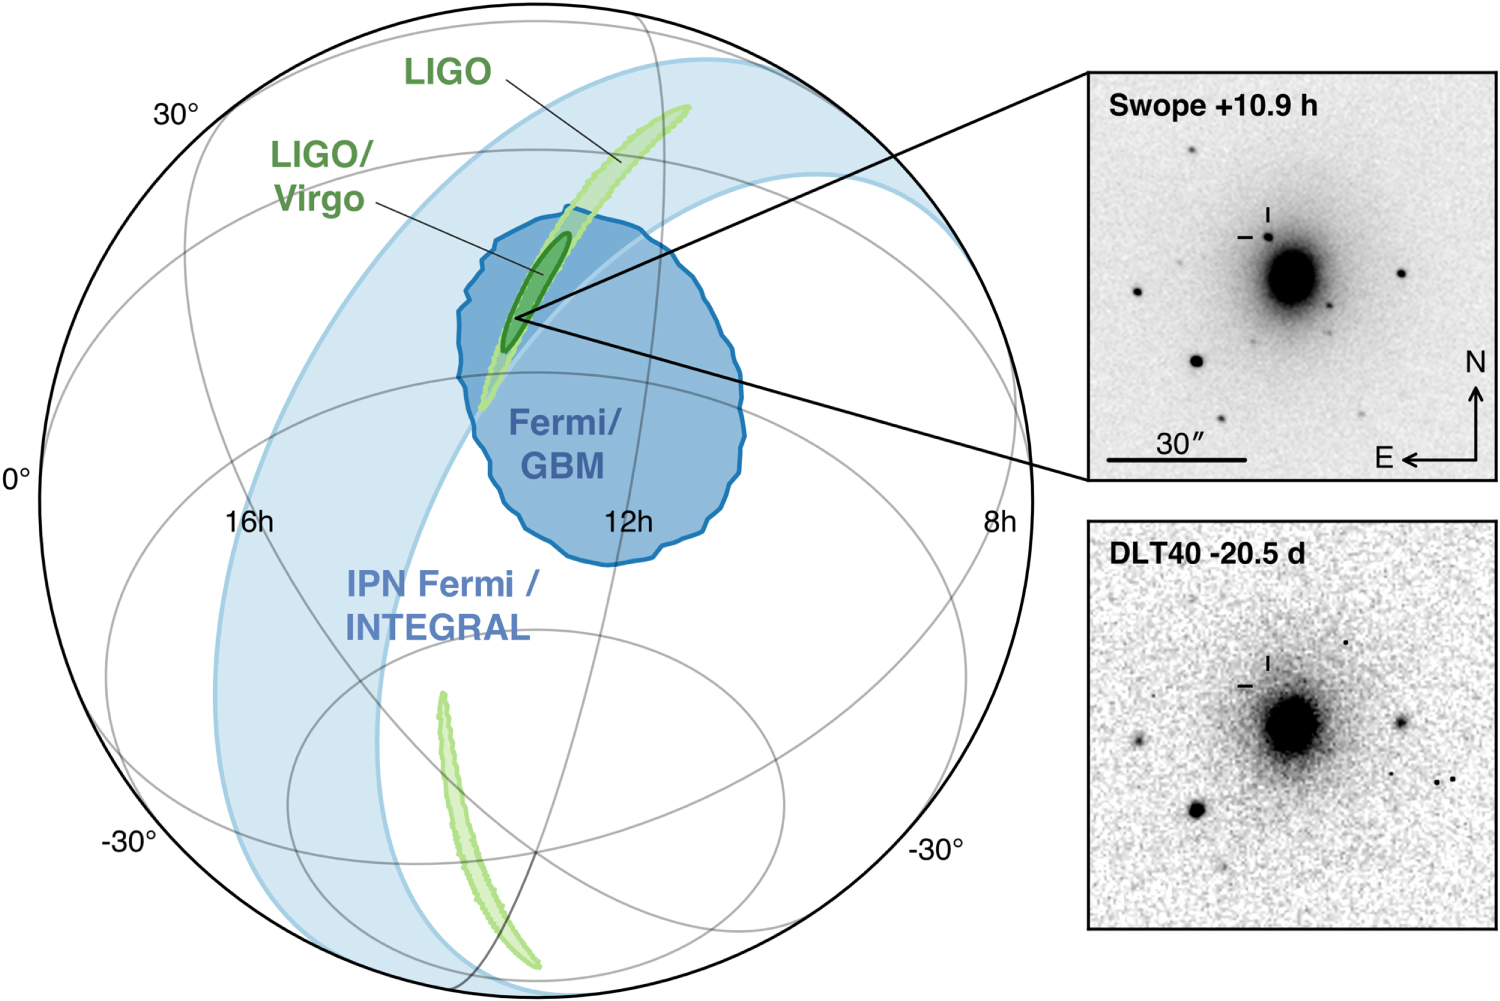
\includegraphics[width=\linewidth]{figures/GW170817_skymap.jpg}
    \caption[Sky localization for the first confirmed detection of a \ac{BNS} merger by the \ac{LVC}.]{Sky localization for the first confirmed detection of a \ac{BNS} merger by the \ac{LVC}. Areas shaded in green are the data products from \texttt{Bayestar} using both \ac{LIGO} alone and \ac{LIGO}/Virgo combined, dark blue are predictions from Fermi/GBM and light blue are predictions from IPN Fermi/INTEGRAL. Black and white images on right-hand side are visible light measurements of a bright event around the galaxy NGC 4993 thought to contain the afterglow of the \ac{BNS} event. This figure was produced by the authors of \cite{2017arXiv171005833L}.}
    \label{fig:GW170817_skylocalization}
\end{figure}

\section{Gravitational Wave Detections}

%
% O1 detections
%

Since it's inception, the \ac{LVC} has carried out several observation runs. Initial operations ran from 2002 to 2010, but no \ac{GW}s were detected during this time period. During the first observing run in the advanced detector era (September 2015 - January 2016), the 
\ac{LVC} detected a total of $3$ \ac{BBH} mergers 
including: GW150914~\cite{PhysRevLett.116.061102}, 
GW151226~\cite{PhysRevLett.116.241103} and 
GW151012~\cite{2010.14527}. GW150914 was the very first detected \ac{BBH} with
an \ac{SNR} value of $\sim 25.1$~\cite{0264-9381-33-21-215004}. GW151012 was originally labeled as a less significant potential GW detection 
(LVT151012) due to its 
high false alarm rate, but was subsequently upgraded to a 
confirmed \ac{GW} event in the GWTC-1 catalogue \cite{1811.12907} because its false alarm rate was less than 1 per 30 days (a threshold determined by the \ac{LVC}). The change in false alarm rate 
for GW151012 can largely be attributed to various improvements made to 
all search algorithms used in the first observation run  
between the initial detection and up to publication 
of the GWTC-1 catalogue paper (for further details, see~\cite{1811.12907,
PhysRevD.102.062003}).

%
% O2 detections
%
During the second observing run (November 2016 - August 2017) the 
\ac{LVC} detected an additional $7$ \ac{BBH}s with total masses between $\sim 18.6 M_\odot$ and $\sim 85.1 M_\odot$. The second observation run excitingly also saw the very first detection of a \ac{BNS} event. The \ac{BNS} event had the highest network \ac{SNR} of any event over all of O1 and O2 ($\sim 32.4$). Interestingly, there was also a large non-astrophysical noise transient which overlapped 
with a portion of the \ac{BNS} event in the \ac{LIGO} Livingston 
detector. This noise transient was successfully mitigated through an 
excising technique known as time-domain gating \cite{PhysRevLett.119.161101}. Approximately 1.7s following GW170817, a \ac{GRB} (GRB170817) was observed 
across multiple wavelengths of the \ac{EM} spectrum over the course of several 
weeks~\cite{2017arXiv171005834L}. The delay between GRB170817 
and GW170817 has been used to place strong constraints on 
various physical phenomena including: the speed of gravity, Lorentz invariance and tests of the equivalence principal~\cite{2017arXiv171005834L}. 
Additionally, given that \ac{GW} 
observations provide direct estimates on the redshift and 
luminosity distance of the 
system, it was shown in ~\cite{Abbott2017} that these observations may be used 
to provide an independent measurement on the Hubble constant 
($H_0 = 70^{+12}_{-8} \mathrm{km s}^{-1} \mathrm{Mpc}^{-1}$).

%
% O3a detections
%
Most recently, during the first half of the third observing run 
(April 2019 - March 2020) the \ac{LVC} collaboration made an 
additional $39$ confirmed \ac{GW} event detections~\cite{1811.12907, 2010.14527}
. The increase in number of detections can largely be attributed to higher sensitivities of the detectors during this observation run over previous runs, with a \ac{BNS} range\footnote{The \ac{BNS} range is a scalar value which is often used to represent the performance of the \ac{LVC} detectors. It 
is quantified by determining the luminosity distance at which a single  
detector could detect a $1.4 \mathrm{M}_\odot$ \ac{BNS} pair with an 
\ac{SNR} $\geq 8$ averaged 
over the sky location and orientation of the source with respect 
to the detector. The range is dependent on a number of factors including: 
source mass/spin and the noise curve~\cite{Abbott_2020} of the detector. See ~\cite{2021CQGra..38e5010C,PhysRevD.47.2198} for more details.} of $108 \mathrm{Mpc}$, $135 \mathrm{Mpc}$ and $45 \mathrm{Mpc}$ for Hanford, Livingston and Virgo respectively. The GWTC-2 catalogue contains detected signals 
with component masses lower and higher 
than the lowest and highest component masses contained in all of 
GWTC-1. The most up-to-date merger rate constraints according to GWTC-2 were also updated to be $\sim 23.9 \mathrm{Gpc}^{-3} \mathrm{yr}^{-1}$ for \ac{BBH}s and $\sim 320 \mathrm{Gpc}^{-3} \mathrm{yr}^{-1}$ for \ac{BNS}s. 

%
% NSBH events
%
In January of 2020, the \ac{LVC} collaboration reported the 
first detection of two  \ac{NSBH} events (GW200105,GW200115)~\cite{Abbott_2021}
. The primary component masses of both events are $\sim 8.9 \mathrm{M}_\odot$ 
and $\sim 5.7 \mathrm{M}_\odot$ respectively, whose mass values are both  
above the maximum allowed mass of a \ac{NS} defined 
in ~\cite{1974PhRvL..32..324R}, 
so may therefore be likely classified as \ac{BH}s. The secondary masses 
of each event were given as $\sim 1.5 \mathrm{M}_\odot$ and $\sim 1.9 \mathrm{M}_\odot$ respectively and were reported to be within the range of 
known \ac{NS}s~\cite{2016arXiv160501665A}.  

%
% Put this in context 
%
As improvements are made to the \ac{LVC} detectors over the coming years, 
it is expected that the rate of detections will increase
dramatically~\cite{2018LRR....21....3A}. It is 
predicted that at design sensitivity, the 
\ac{LVC} will observe $\mathcal{O}(100s)$ of events 
per year~\cite{2018LRR....21....3A}. Current 
methods for both \ac{GW} detection and parameter estimation, 
while optimal in many cases, are often computationally expensive~\cite{}. 
Algorithms which produce estimates on source parameter values of 
\ac{GW} signals can take upwards of weeks to run (see Tab.~\ref{tab:o3_events_runtime_1} and
Tab.~\ref{tab:o3_events_runtime_2} in Ch.~\ref{ch:chap_5}).
Given that follow-up observations of \ac{GW} \ac{EM} components 
heavily depend upon \ac{GW} sky location alerts 
from the \ac{LVC} and 
the rapid decay of \ac{GW} \ac{EM} signatures~\cite{2017arXiv171005833L}, 
there is an urgent need for faster techniques which can not only 
identify the presence of \ac{GW} signals in detector data, 
but also identify source parameter values like the sky location 
of a \ac{GW} event. 

% 
% Transition to GR, GWs and the rest of the thesis
%
%All of these detections are built upon the foundations of \ac{GR}, 
%\ac{LVC} detector design/implementation, current \ac{GW} search methods and 
%\ac{GW} parameter estimation techniques. As outlined, these concepts were 
%discsussed in detail over the course of this chapter.  as well as motivate 
%the urgent need for the development of more efficient 
%search and parameter estimation algorithms. 

\section{Summary}

The chapter opens 
by discussing the detections made by the \ac{LVC} in the past 3 
observation runs and how those detections have been used to 
further our understanding of cosmology, astrophysics and \ac{GW} astronomy.
A brief introduction to Einstein's Field Equations and how those field equations lead to the prediction that \ac{GW}s exist was provided. It was 
shown that various sources are able to produce \ac{GW}s and it was described 
how the \ac{LVC} detectors physically operate to detect such signals. The 
search techniques for all source signals was described, along with a 
description on how predictions are generated on the 
underlying source parameters of \ac{GW} signals. From the descriptions 
of the search and parameter estimation techniques given in Sec.~\ref{sec:matched_filtering} and Sec.
~\ref{sec:bayesian_inference} it was shown that while optimal under Gaussian-noise conditions, standard 
approaches used by the \ac{LVC} are computationally expensive to 
run. This is especially problematic given the large number of 
expected signals the \ac{LVC} will see in the coming years, with 
the additional need of alerting \ac{EM} partners in low-latency due 
to short-lived \ac{GW} \ac{EM} counterparts. Given the urgent need 
for low-latency tools to perform both \ac{GW} detection and \ac{GW} 
parameter estimation, we will show in the subsequent chapters (Ch.~\ref{ch:chap_4}, Ch.~\ref{ch:chap_5}) how recent advances in  
the field of \ac{ML} may be applied in order to solve these problems. 
In the next chapter (Ch.~\ref{ch:chap_2}), we will describe the basics 
of \ac{ML}, as well as provide detailed descriptions of 
the \ac{ML} algorithms used in this thesis.